\documentclass[a4paper]{book}

\usepackage{afterpage}
\usepackage[hypcap=false]{caption}
\usepackage{enumitem}	% 定制enumerate标号
\usepackage{geometry}
\geometry{%
	left=2cm,%
	right=2cm,%
	top=2cm,%
	bottom=2cm,%
	bindingoffset=0cm
}
\usepackage{hyperref}
\hypersetup{
    colorlinks=true,            %链接颜色
    linkcolor=blue,             %内部链接
    filecolor=magenta,          %本地文档
    urlcolor=cyan,              %网址链接
    pdftitle={Overleaf Example},
    pdfpagemode=FullScreen,
}
\usepackage[none]{hyphenat}	% 阻止长单词分在两行
\usepackage{longtable}
\usepackage{mathrsfs}	% 提供\mathscr字体
\usepackage[version=4]{mhchem}
\usepackage{multirow}
\usepackage{subcaption}

\RequirePackage[many]{tcolorbox}
\tcbset{
    boxed title style={colback=magenta},
	breakable,
	enhanced,
	sharp corners,
	attach boxed title to top left={yshift=-\tcboxedtitleheight,  yshifttext=-.75\baselineskip},
	boxed title style={boxsep=1pt,sharp corners},
    fonttitle=\bfseries\sffamily,
}

\definecolor{skyblue}{rgb}{0.54, 0.81, 0.94}

\newtcolorbox[auto counter, number within=chapter, number format=\arabic]{exercise}[1][]{
    title={Exercise~\thetcbcounter},
    colframe=skyblue,
    colback=skyblue!12!white,
    boxed title style={colback=skyblue},
    overlay unbroken and first={
        \node[below right,font=\small,color=skyblue,text width=.8\linewidth]
        at (title.north east) {#1};
    }
}

\newtcolorbox[auto counter, number within=chapter, number format=\arabic]{solution}[1][]{
%    top=2ex,
%    boxrule=0pt,
%    leftrule=1.4pt,
    title={Solution~\thetcbcounter},
    colframe=teal!60!green,
    colback=green!12!white,
    boxed title style={colback=teal!60!green},
    overlay unbroken and first={
        \node[below right,font=\small,color=red,text width=.8\linewidth]
        at (title.north east) {#1};
    }
}

\newcommand{\AO}{{\rm AO}}
\newcommand{\Heff}{H^{\rm eff,\pi}}
\newcommand{\Hp}{H^\prime}
\newcommand{\Sp}{S^\prime}
\newcommand{\RRR}{{\rm R}^3}
\newcommand\Figref[1]{Fig \ref{#1}}
\newcommand\Tableref[1]{Table \ref{#1}}
\newcommand{\orb}[1]{{\rm #1}}
\newcommand{\orbp}{\orb{p}}

\allowdisplaybreaks

\begin{document}

	\setcounter{chapter}{10}

	\begin{exercise}
		For the following molecules, determine the point group and the symmetry of the MOs for the $\pi$-electrons, and, using H{\"u}ckel theory, obtain the MOs and orbital energies:
		\begin{enumerate}[label=(\alph*)]
		\item {\it trans}-1,3-butadiene,
		\item ethylene,
		\item cyclobutadiene,
		\item cyclopentadienyl radical $\ce{C5H5}$,
		\item naphthalene,
		\item phenanthrene.
		\end{enumerate}
	\end{exercise}

	\begin{solution}

		\begin{enumerate}[label=(\alph*)]
	
		\item % trans-1,3-butadiene.tex

\item Firstly, it is easy to find that {\it trans}-1,3-butadiene belongs to the point group $\mathscr{C}_{\rm 2h}$, whose character table is listed below.
		\begin{center}
		\setlength{\abovecaptionskip}{-0.1em}
		\captionof{table}{The character table for the $\mathscr{C}_{\rm 2h}$ point group.}
		\begin{tabular}{ccccc}\hline
	$\mathscr{C}_{\rm 2h}$ & $E$ & $C_2$ & $i$ & $\sigma_h$ \\ \hline
			$A_g$	&	1	&	1	&	1	&	1	\\
			$B_g$	&	1	&	-1	&	1	&	-1	\\
			$A_u$	&	1	&	1	&	-1	&	-1	\\
			$B_u$ 	&	1	&	-1	&	-1	&	1	\\ \hline
		\end{tabular}
		\setlength{\belowcaptionskip}{-0.2em}
		\end{center}
		
		Secondly, we mark all carbon atoms as follows.
		\begin{center}
		
\includegraphics[scale=1.0]{./structures/exercise_1/trans-1,3-butadiene/0.png}
		\setlength{\abovecaptionskip}{-0.3em}
		\captionof{figure}{The order of carbon atoms in {\it trans}-1,3-butadiene.}
		\setlength{\belowcaptionskip}{-0.8em}
		\end{center}				

		For $\pi$-electron atomic orbitals' representation $\Gamma^{\rm AO}$, its following characters is listed below.
		\begin{center}
		\setlength{\abovecaptionskip}{-0.3em}
		\captionof{table}{The character of the $\pi$-electron atomic orbitals' representation $\Gamma^{\rm AO}$.}
		\begin{tabular}{ccccc}\hline
	$\mathscr{C}_{\rm 2h}$ & $E$ & $C_2$ & $i$ & $\sigma_h$ \\ \hline
	$\chi^{\AO}(C_i)$	&	4	&	0	&	0	&	-4	\\ \hline
		\end{tabular}\vspace*{-0.5em}
		\end{center}
		
		Relevant reduction coefficients are
		\begin{align*}
		a_g &= \frac{1}{4} \sum_{R} \chi^{\AO}(R) \chi^{A_g}(R) = \frac{1}{4} \left[ 1 \times 4 \times 1 + 1 \times 0 \times 1 + 1 \times 0 \times 1 + 1 \times (-4) \times 1 \right] = 0, \\
		b_g &= \frac{1}{4} \sum_{R} \chi^{\AO}(R) \chi^{B_g}(R) = \frac{1}{4} \left[ 1 \times 4 \times 1 + 1 \times 0 \times (-1) + 1 \times 0 \times 1 + 1 \times (-4) \times (-1) \right] = 2, \\
		a_u &= \frac{1}{4} \sum_{R} \chi^{\AO}(R) \chi^{A_u}(R) = \frac{1}{4} \left[ 1 \times 4 \times 1 + 1 \times 0 \times 1 + 1 \times 0 \times (-1) + 1 \times (-4) \times (-1) \right] = 2, \\
		b_u &= \frac{1}{4} \sum_{R} \chi^{\AO}(R) \chi^{B_u}(R) = \frac{1}{4} \left[ 1 \times 4 \times 1 + 1 \times 0 \times (-1) + 1 \times 0 \times (-1) + 1 \times (-4) \times 1 \right] = 0.
		\end{align*}
		
		Thus, we arrive at
		\begin{equation*}
			\Gamma^{\AO} = 2 \Gamma^{B_g} \oplus 2 \Gamma^{A_u}.
		\end{equation*}
		We conclude that there are two basis functions in the irreducible representation $\Gamma^{B_g}$ and $\Gamma^{A_u}$, respectively. Thus, to describe the effect of $O_R$, two suitable $2 \orbp_z$ atomic orbitals $\phi_i$ is enough.
		
		Thirdly, we inspect the transformation of $\phi_i$ under $O_R$ for the {\it trans}-1,3-butadiene, whose information is recorded below. We only list two $\phi_1$ and $\phi_2$, which is enough in current case.
		\begin{center}
		\setlength{\abovecaptionskip}{0em}
		\captionof{table}{Transformation of $\phi_i$ under $O_R$ for the {\it trans}-1,3-butadiene.}
		\begin{tabular}{ccccc}\hline
	$\mathscr{C}_{\rm 2h}$ & $O_E$ & $O_{C_2}$ & $O_i$ & $O_{\sigma_h}$ \\ \hline
			$\phi_1$	&	$\phi_1$	&	$\phi_4$	&	$-\phi_4$	&	$-\phi_1$	\\
			$\phi_2$	&	$\phi_2$	&	$\phi_3$	&	$-\phi_3$	&	$-\phi_2$	\\	\hline
		\end{tabular}
		\setlength{\belowcaptionskip}{0.5em}
		\end{center}
		
		For the irreducible representation $\Gamma^{B_g}$,
		\begin{align*}
		P^{B_g}\phi_1 &= \sum_{R} \chi^{B_g}(R) O_R \phi_1 = (O_E - O_{C_2} + O_{i} - O_{\sigma_h})\phi_1 = 2(\phi_1-\phi_4) , \\
		P^{B_g}\phi_2 &= \sum_{R} \chi^{B_g}(R) O_R \phi_2 = (O_E - O_{C_2} + O_{i} - O_{\sigma_h})\phi_2 = 2(\phi_2-\phi_3) .
		\end{align*}
		It is easy to find that they are mutually orthogonal. They can be normalized to
		\begin{align*}
		\phi^\prime_1 &= \frac{1}{\sqrt{2}} (\phi_1-\phi_4) , \\
		\phi^\prime_2 &= \frac{1}{\sqrt{2}} (\phi_2-\phi_3) .
		\end{align*}
		
		Then, the effective Hamitonian matrix elements for $\pi$ electrons can be calculated,
		\begin{align*}
		\Hp_{11} &= \int_{\RRR} \frac{1}{\sqrt{2}}(\phi_1-\phi_4) \Heff \frac{1}{\sqrt{2}}(\phi_1-\phi_4) = \frac{1}{2} (\alpha + 0 + 0 + \alpha) = \alpha, \\
		\Hp_{12} &= \int_{\RRR} \frac{1}{\sqrt{2}}(\phi_1-\phi_4) \Heff \frac{1}{\sqrt{2}}(\phi_2-\phi_3) = \frac{1}{2} (\beta - 0 - 0 + \beta) = \beta, \\
		\Hp_{22} &= \int_{\RRR} \frac{1}{\sqrt{2}}(\phi_2-\phi_3) \Heff \frac{1}{\sqrt{2}}(\phi_2-\phi_3) = \frac{1}{2} (\alpha - \beta - \beta + \alpha) = \alpha - \beta,
		\end{align*}
		viz.
		\begin{equation*}
			\Hp_{B_g} = \begin{pmatrix}
				\alpha	&	\beta \\ \beta & \alpha - \beta 
			\end{pmatrix}.
		\end{equation*}
		Next,
		\begin{align*}
			\det(\Hp_{B_g}-\varepsilon^\pi \Sp_{B_g}) = \begin{vmatrix}	
			\alpha-\varepsilon^\pi	&	\beta \\ 
			\beta & \alpha - \beta -\varepsilon^\pi	
\end{vmatrix} = \beta^2
\begin{vmatrix}
			x & 1 \\ 1 & x -1			
			\end{vmatrix} = \beta^2 ( x^x - x - 1 ) = 0,
		\end{align*}
		where
		\begin{equation*}
			x = \frac{\alpha-\varepsilon^\pi}{\beta}.
		\end{equation*}
		Current discriminant is
		\begin{equation*}
			\Delta_{B_g} = (-1)^2 - 4 \times 1 \times (-1) = 5,
		\end{equation*}				
		and then two roots are
		\begin{equation*}
			x_1 = \frac{1+\sqrt{5}}{2}, \quad x_2 = \frac{1-\sqrt{5}}{2},
		\end{equation*}
		which equal to	
		\begin{align}
			\varepsilon_1 &= \alpha - x_1 \beta = \alpha - \frac{1+\sqrt{5}}{2} \beta \approx \alpha - 1.618 \beta , \\
			\varepsilon_2 &= \alpha - x_2 \beta = \alpha - \frac{1-\sqrt{5}}{2} \beta = \alpha + \frac{\sqrt{5}-1}{2} \beta \approx \alpha + 0.618 \beta .
		\end{align}
		
		For $\Hp_{B_g}-\varepsilon^\pi_1 \Sp_{B_g}$, its reduced row echelon form is
		\begin{equation*}
			\begin{pmatrix}
				1	& \frac{-1+\sqrt{5}}{2}	\\	0	&	0
			\end{pmatrix},
		\end{equation*}
		which means
		\begin{equation*}
			\Phi_1 = -\frac{\sqrt{5}-1}{2}\phi^\prime_1 + \phi^\prime_2.
		\end{equation*}
		The sum of squares of coefficients is
		\begin{equation*}
			\sum_{i} c^2_i = (-\frac{\sqrt{5}-1}{2})^2 + 1^2 = \frac{5-\sqrt{5}}{2}.
		\end{equation*}
		
		Thus, we know
		\begin{align}
			\Phi^\pi_1 &= \sqrt{ \frac{2}{5-\sqrt{5}} } \Phi_1 = -\frac{\sqrt{5}-1}{2}\phi^\prime_1 + \phi^\prime_2 = - \sqrt{\frac{\sqrt{5}-1}{2\sqrt{5}}} \phi^\prime_1 + \sqrt{\frac{\sqrt{5}+1}{2\sqrt{5}}} \phi^\prime_2	\notag \\
			&= - \frac{1}{2}\sqrt{\frac{\sqrt{5}-1}{\sqrt{5}}}\phi_1  + \frac{1}{2}\sqrt{\frac{\sqrt{5}+1}{\sqrt{5}}} \phi_2 - \frac{1}{2}\sqrt{\frac{\sqrt{5}+1}{\sqrt{5}}} \phi_3 + \frac{1}{2}\sqrt{\frac{\sqrt{5}-1}{\sqrt{5}}} \phi_4 \notag \\
			&\approx -0.3717 \phi_1 + 0.6015 \phi_2 - 0.6015 \phi_3 + 0.3717 \phi_4.
		\end{align}
		
		Similarly, the reduced row echelon form of $\Hp_{B_g}-\varepsilon^\pi_2 \Sp_{B_g}$ is
		\begin{equation*}
			\begin{pmatrix}
				1	& \frac{-1-\sqrt{5}}{2}	\\	0	&	0
			\end{pmatrix},
		\end{equation*}		
		which means
		\begin{equation*}
			\Phi_2 = \frac{\sqrt{5}+1}{2}\phi^\prime_1 + \phi^\prime_2.
		\end{equation*}
		And then,
		\begin{align}
			\Phi^\pi_2 &= \sqrt{ \frac{2}{5+\sqrt{5}} } \Phi_2 = \frac{\sqrt{5}+1}{2}\phi^\prime_1 + \phi^\prime_2 = \sqrt{\frac{\sqrt{5}+1}{2\sqrt{5}}} \phi^\prime_1 + \sqrt{\frac{\sqrt{5}-1}{2\sqrt{5}}} \phi^\prime_2	\notag \\
			&= \frac{1}{2}\sqrt{\frac{\sqrt{5}+1}{\sqrt{5}}}\phi_1  + \frac{1}{2}\sqrt{\frac{\sqrt{5}-1}{\sqrt{5}}} \phi_2 - \frac{1}{2}\sqrt{\frac{\sqrt{5}-1}{\sqrt{5}}} \phi_3 - \frac{1}{2}\sqrt{\frac{\sqrt{5}+1}{\sqrt{5}}} \phi_4 \notag \\
			&\approx 0.6015\phi_1 + 0.3717 \phi_2 - 0.3717 \phi_3 -  0.6015\phi_4.
		\end{align}
		
		In conclusion, for the irreducible representation $\Gamma^{B_g}$, relevant results are listed below.
		
		\begin{center}
		\setlength{\abovecaptionskip}{-0.5em}
		\captionof{table}{The H{\"u}ckel MOs in the irreducible representation $\Gamma^{B_g}$ of {\it trans}-1,3-butadiene.}
		\begin{tabular}{ccc}\hline
		  order	&	eigenvalue		& 	eigenfunction	\\ \hline
			1	&$\alpha-1.618\beta$& 	$-0.3717 \phi_1 + 0.6015 \phi_2 - 0.6015 \phi_3 + 0.3717 \phi_4$ \\
			2	&$\alpha+0.618\beta$& 	$0.6015\phi_1 + 0.3717 \phi_2 - 0.3717 \phi_3 -  0.6015\phi_4$\\ \hline
		\end{tabular}
		\end{center}
		
		In the same way, for the irreducible representation $\Gamma^{A_u}$,
		\begin{align*}
		P^{A_u}\phi_1 &= \sum_{R} \chi^{A_u}(R) O_R \phi_1 = (O_E + O_{C_2} - O_{i} - O_{\sigma_h})\phi_1 = 2(\phi_1+\phi_4) , \\
		P^{A_u}\phi_2 &= \sum_{R} \chi^{A_u}(R) O_R \phi_2 = (O_E + O_{C_2} - O_{i} - O_{\sigma_h})\phi_2 = 2(\phi_2+\phi_3) .
		\end{align*}
		It is easy to find that they are mutually orthogonal, too. They can be normalized to
		\begin{align*}
		\phi^\prime_3 &= \frac{1}{\sqrt{2}} (\phi_1+\phi_4) , \\
		\phi^\prime_4 &= \frac{1}{\sqrt{2}} (\phi_2+\phi_3) .
		\end{align*}
		Then, the effective Hamiltonian can be constructed, viz.
		\begin{equation*}
			\Hp_{A_u} = \begin{pmatrix}
				\alpha	&	\beta \\ \beta & \alpha + \beta 
			\end{pmatrix}.
		\end{equation*}
		Next,
		\begin{align*}
			\det(\Hp_{A_u}-\varepsilon^\pi \Sp_{A_u}) = \begin{vmatrix}	
			\alpha-\varepsilon^\pi	&	\beta \\ 
			\beta & \alpha + \beta -\varepsilon^\pi	
\end{vmatrix} = \beta^2
\begin{vmatrix}
			x & 1 \\ 1 & x +1			
			\end{vmatrix} = \beta^2 ( x^x + x - 1 ) = 0.
		\end{align*}
		Current discriminant is
		\begin{equation*}
			\Delta_{A_u} = 1^2 - 4 \times 1 \times (-1) = 5,
		\end{equation*}		
		and then two roots are
		\begin{equation*}
			x_3 = \frac{-1+\sqrt{5}}{2}, \quad x_4 = \frac{-1-\sqrt{5}}{2},
		\end{equation*}
		which equal to
		\begin{align}
			\varepsilon_3 &= \alpha - x_3 \beta = \alpha - \frac{-1+\sqrt{5}}{2} \beta \approx \alpha - 0.618 \beta , \\
			\varepsilon_4 &= \alpha - x_4 \beta = \alpha - \frac{-1-\sqrt{5}}{2} \beta = \alpha + \frac{\sqrt{5}+1}{2} \beta \approx \alpha + 1.618 \beta .
		\end{align}
		
		For $\Hp_{A_u}-\varepsilon^\pi_3 \Sp_{A_u}$, its reduced row echelon form is
		\begin{equation*}
			\begin{pmatrix}
				1	& \frac{1+\sqrt{5}}{2}	\\	0	&	0
			\end{pmatrix},
		\end{equation*}		
		which means
		\begin{equation*}
			\Phi_3 = -\frac{\sqrt{5}+1}{2}\phi^\prime_3 + \phi^\prime_4.
		\end{equation*}
		Thus,
		\begin{align}
			\Phi^\pi_3 &= \sqrt{ \frac{2}{5+\sqrt{5}} } \Phi_3 = -\sqrt{\frac{\sqrt{5}+1}{2\sqrt{5}}} \phi^\prime_3 + \sqrt{\frac{\sqrt{5}-1}{2\sqrt{5}}} \phi^\prime_4 \notag	\\
			&= -\frac{1}{2}\sqrt{\frac{\sqrt{5}+1}{\sqrt{5}}}\phi_1  + \frac{1}{2}\sqrt{\frac{\sqrt{5}-1}{\sqrt{5}}} \phi_2 + \frac{1}{2}\sqrt{\frac{\sqrt{5}-1}{\sqrt{5}}} \phi_3 - \frac{1}{2}\sqrt{\frac{\sqrt{5}+1}{\sqrt{5}}} \phi_4 \notag \\
			&\approx -0.6015 \phi_1 + 0.3717 \phi_2 + 0.3717 \phi_3 - 0.6015 \phi_4.
		\end{align}
		
		For $\Hp_{A_u}-\varepsilon^\pi_4 \Sp_{A_u}$, its reduced row echelon form is
		\begin{equation*}
			\begin{pmatrix}
				1	& \frac{1-\sqrt{5}}{2}	\\	0	&	0
			\end{pmatrix},
		\end{equation*}		
		which means
		\begin{equation*}
			\Phi_4 = \frac{\sqrt{5}-1}{2}\phi^\prime_3 + \phi^\prime_4.
		\end{equation*}
		Thus,		
		\begin{align}
			\Phi^\pi_4 &= \sqrt{ \frac{2}{5-\sqrt{5}} } \Phi_4 = \sqrt{\frac{\sqrt{5}-1}{2\sqrt{5}}} \phi^\prime_3 + \sqrt{\frac{\sqrt{5}+1}{2\sqrt{5}}} \phi^\prime_4 \notag	\\
			&= \frac{1}{2}\sqrt{\frac{\sqrt{5}-1}{\sqrt{5}}}\phi_1  + \frac{1}{2}\sqrt{\frac{\sqrt{5}+1}{\sqrt{5}}} \phi_2 + \frac{1}{2}\sqrt{\frac{\sqrt{5}+1}{\sqrt{5}}} \phi_3 + \frac{1}{2}\sqrt{\frac{\sqrt{5}-1}{\sqrt{5}}} \phi_4 \notag \\
			&\approx 0.3717 \phi_1 + 0.6015 \phi_2 + 0.6015 \phi_3 + 0.3717 \phi_4.
		\end{align}
		
		In conclusion, for the irreducible representation $\Gamma^{A_u}$, relevant results are listed below.
		
		\begin{center}
		\setlength{\abovecaptionskip}{-0.5em}
		\captionof{table}{The H{\"u}ckel MOs in the irreducible representation $\Gamma^{A_u}$ of {\it trans}-1,3-butadiene.}
		\begin{tabular}{ccc}\hline
		  order	&	eigenvalue		& 	eigenfunction	\\ \hline
			1	&$\alpha-0.618\beta$& 	$-0.6015 \phi_1 + 0.3717 \phi_2 + 0.3717 \phi_3 - 0.6015 \phi_4$ \\
			2	&$\alpha+1.618\beta$& 	$0.3717\phi_1 + 0.6015 \phi_2 +0.6015 \phi_3 + 0.3717\phi_4$  \\	 \hline
		\end{tabular}
		\end{center}
		
		Now, we have obtained all results, which are shown as following.
		
		\begin{center}
		\setlength{\abovecaptionskip}{-0.5em}
		\captionof{table}{The H{\"u}ckel MOs in all irreducible representations of {\it trans}-1,3-butadiene.}
		\begin{tabular}{ccccccc}\hline
		order 	& orbital energy & irrep & $c_1$ & $c_2$ & $c_3$ &$c_4$ \\ \hline
			1	&	$\alpha+1.618\beta$	&	$A_u$	&	0.3717	&	0.6015	&	0.6015	&	0.3717	\\
			2	&	$\alpha+0.618\beta$	&	$B_g$	&	0.6015	&	0.3717	&	-0.3717	&	-0.6015	\\
			3	&	$\alpha-0.618\beta$	&	$A_u$	&	0.6015	&	-0.3717	&	-0.3717	&	0.6015	\\
			4	&	$\alpha-1.618\beta$	&	$B_g$	&	0.3717	&	-0.6015	&	0.6015	&	-0.3717	\\ \hline
		\end{tabular}
		\end{center}
		
		Besides, their phase diagrams have been painted in \Figref{fig:phase_diagram_1}. They obey the rule that the less nodal planes are, the lower orbital energy is.
		
		\begin{center}
		\begin{tabular}{cccc}
			\begin{minipage}[t]{0.22\linewidth}
			\centering
			\setlength{\abovecaptionskip}{0.5em}
			\includegraphics[scale=0.95]{./structures/exercise_1/trans-1,3-butadiene/4.png}
			\captionof*{figure}{$\varepsilon = \alpha + 1.618\beta$}
			\end{minipage} & 
			\begin{minipage}[t]{0.18\linewidth}
			\setlength{\abovecaptionskip}{0.5em}
			\includegraphics[scale=0.95]{./structures/exercise_1/trans-1,3-butadiene/2.png}
			\captionof*{figure}{$\varepsilon = \alpha + 0.618\beta$}
			\end{minipage} &
			\begin{minipage}[t]{0.22\linewidth}
			\centering
			\setlength{\abovecaptionskip}{0.5em}
			\includegraphics[scale=0.95]{./structures/exercise_1/trans-1,3-butadiene/3.png}
			\captionof*{figure}{$\varepsilon = \alpha - 0.618\beta$}
			\end{minipage} & 
			\begin{minipage}[t]{0.18\linewidth}
			\setlength{\abovecaptionskip}{0.5em}
			\includegraphics[scale=0.95]{./structures/exercise_1/trans-1,3-butadiene/1.png}
			\captionof*{figure}{$\varepsilon = \alpha - 1.618\beta$}
			\end{minipage}
		\end{tabular}				
		\captionof{figure}{Phase diagrams of these H{\"u}ckel MOs of {\it trans}-1,3-butadiene. Black bubbles mean plus phase while white ones mean minus phase. The color is used just for determining relative phase.}\label{fig:phase_diagram_1}
		\end{center}
		
		In the end, we conclude that for {\it trans}-1,3-butadiene, its ground state $\pi$-electron configuration is $(a_u)^2(b_g)^2$ and its delocalization energy is $2\times(1.618\beta+0.618\beta)-4\beta=0.472\beta$.
		
		\item 		
		bbbbbbbbbbbbbbbbbbbbbbbbbbbbb
		
		\begin{center}
		\begin{tabular}{ccccc}\hline
	$\mathscr{D}_{\rm 2}$ & $E$ & $C_{2z}$ & $C_{2y}$ & $C_{2x}$ \\ \hline
			$A$		&	1	&	1	&	1	&	1	\\
			$B_1$	&	1	&	1	&	-1	&	-1	\\
			$B_2$	&	1	&	-1	&	1	&	-1	\\
			$B_3$ 	&	1	&	-1	&	-1	&	1	\\ \hline
		\end{tabular}
		\end{center}
		
		
		\begin{center}
		\begin{tabular}{ccccc}\hline
	$\mathscr{D}_{\rm 2}$ & $E$ & $C_{2z}$ & $C_{2y}$ & $C_{2x}$  \\ \hline
	$\chi^{\AO}(C_i)$	&	2	&	0	&	0	&	-2	\\ \hline
		\end{tabular}
		\end{center}
		
		\begin{align*}
		a &= \frac{1}{4} \sum_{R} \chi^{\AO}(R) \chi^{A}(R) = \frac{1}{4} \left[ 1 \times 2 \times 1 + 1 \times 0 \times 1 + 1 \times 0 \times 1 + 1 \times (-2) \times 1 \right] = 0, \\
		b_1	&= \frac{1}{4} \sum_{R} \chi^{\AO}(R) \chi^{B_1}(R) = \frac{1}{4} \left[ 1 \times 2 \times 1 + 1 \times 0 \times 1 + 1 \times 0 \times (-1) + 1 \times (-2) \times (-1) \right] = 1, \\
		b_2	&= \frac{1}{4} \sum_{R} \chi^{\AO}(R) \chi^{B_2}(R) = \frac{1}{4} \left[ 1 \times 2 \times 1 + 1 \times 0 \times (-1) + 1 \times 0 \times 1 + 1 \times (-2) \times (-1) \right] = 1, \\
		b_3	&= \frac{1}{4} \sum_{R} \chi^{\AO}(R) \chi^{B_3}(R) = \frac{1}{4} \left[ 1 \times 2 \times 1 + 1 \times 0 \times (-1) + 1 \times 0 \times (-1) + 1 \times (-2) \times 1 \right] = 0.
		\end{align*}
		
		\begin{equation*}
			\Gamma^{\AO} = \Gamma^{B_1} \oplus \Gamma^{B_2}.
		\end{equation*}
		
		\begin{center}
		\begin{tabular}{ccccc}\hline
	$\mathscr{D}_{\rm 2}$ & $E$ & $C_{2z}$ & $C_{2y}$ & $C_{2x}$ \\ \hline
			$\phi_1$	&	$\phi_1$	&	$\phi_2$	&	$-\phi_2$	&	$-\phi_1$	\\	\hline
		\end{tabular}
		\end{center}
		
		\begin{equation*}
		P^{B_1}\phi_1 = \sum_{R} \chi^{B_1}(R) O_R \phi_1 = (O_E + O_{C_{2z}} - O_{C_{2y}} - O_{C_{2x}})\phi_1 = \phi_1 +\phi_2 - (-\phi_2) - (-\phi_1) = 2(\phi_1 + \phi_2) .
		\end{equation*}
		
		\begin{equation*}
		\phi^\prime_1 = \frac{1}{2}(\phi_1 + \phi_2) .
		\end{equation*}
		
		\begin{equation*}
			\Heff = ( \alpha + \beta ).
		\end{equation*}
		
		\begin{align}
			\Psi^pi_1 &= \phi^\prime_1 = \frac{1}{2}(\phi_1 + \phi_2) \\
			&\approx 0.7071 \phi_1 + 0.7071 \phi_2.
		\end{align}
		
		
		\begin{equation*}
		P^{B_2}\phi_1 = \sum_{R} \chi^{B_2}(R) O_R \phi_1 = (O_E - O_{C_{2z}} + O_{C_{2y}} - O_{C_{2x}})\phi_1 = \phi_1 - \phi_2 + (-\phi_2) + (-\phi_1) = 2(\phi_1 - \phi_2) .
		\end{equation*}
		
		\begin{equation*}
		\phi^\prime_2 = \frac{1}{2}(\phi_1 - \phi_2) .
		\end{equation*}
		
		\begin{equation*}
			\Heff = ( \alpha - \beta ).
		\end{equation*}
		
		\begin{align}
			\Psi^pi_1 &= \phi^\prime_1 = \frac{1}{2}(\phi_1 - \phi_2) \\
			&\approx 0.7071 \phi_1 - 0.7071 \phi_2.
		\end{align}
		
		Thus, we obtain all results, which are shown as following.
		
		\begin{center}
		\begin{tabular}{ccccc}\hline
		order 	& orbital energy & irrep & $c_1$ & $c_2$ \\ \hline
			1	&	$\alpha+\beta$	&	$B_1$	&	0.7071	&	-0.7071	\\
			2	&	$\alpha-\beta$	&	$B_2$	&	0.7071	&	-0.7071	\\ \hline
		\end{tabular}
		\end{center}
		
		\begin{center}
		\begin{tabular}{cccc}
			\begin{minipage}[t]{0.2\linewidth}
			\centering
			\setlength{\abovecaptionskip}{0.5em}
			\includegraphics[scale=1]{./structures/exercise_1/ethylene/1.png}
			\captionof*{figure}{$\varepsilon = \alpha + \beta$}
			\end{minipage} & 
			\begin{minipage}[t]{0.11\linewidth}
			\setlength{\abovecaptionskip}{0.5em}
			\includegraphics[scale=1]{./structures/exercise_1/ethylene/2.png}
			\captionof*{figure}{$\varepsilon = \alpha - \beta$}
			\end{minipage}
		\end{tabular}				
		\captionof{figure}{Phase diagrams of these H{\"u}ckel MOs. Black bubbles mean plus phase while white ones mean minus phase. The color is used just for determining relative phase.}\label{fig:phase_diagram_2}
		\end{center}
		
		\item This solution is designed for cyclobutadiene anion instead of just cyclobutadiene which is the prototypical antiaromatic hydrocarbon with 4 $\pi$ electrons. Its rectangular structure is the result of a pseudo-(or second order) Jahn–Teller effect, which distorts the molecule and lowers its symmetry, converting the triplet to a singlet ground state. This distortion indicates that the $\pi$ electrons are localized, in agreement with H{\"u}ckel's rule which predicts that a $\pi$-system of 4 electrons is not aromatic. This information is excerpted from \url{https://en.wikipedia.org/wiki/Cyclobutadiene}.
		
		Firstly, it is easy find that cyclobutadiene anion belongs to the point group $\mathscr{D}_{\rm 4h}$. However, it has only 4 $\pi$-electrons. Just $\mathscr{D}_{\rm 4}$ is good enough and its character table is shown in \Tableref{tab:chatab_3}.
		\begin{center}
		\setlength{\abovecaptionskip}{0em}
		\captionof{table}{The character table for the $\mathscr{D}_{\rm 4}$ point group.}\label{tab:chatab_3}
		\begin{tabular}{cccccc}\hline
	$\mathscr{D}_{\rm 4}$ & $E$ & $2C_4$ &	$C_2$	& $2C^\prime_2$ & $2C^{\prime\prime}_2$ \\ \hline
			$A_1$	&	1	&	1	&	1	&	1	&	1	\\
			$A_1$	&	1	&	1	&	1	&	-1	&	-1	\\
			$B_1$	&	1	&	-1	&	1	&	1	&	-1	\\
			$B_2$	&	1	&	-1	&	1	&	-1	&	1	\\
			$E$ 	&	2	&	0	&	-2	&	0	&	0\\ \hline
		\end{tabular}
		\end{center}
		
		Secondly, we mark all carbon atoms as follows.
		\begin{center}
		\setlength{\abovecaptionskip}{-0.5em}
		
\includegraphics[scale=1.0]{./structures/exercise_1/cyclobutadiene_anion/0.png}
		\captionof{figure}{The order of carbon atoms in the cyclobutadiene anion.}\label{fig:case3}
		\end{center}
		
		For $\pi$-electron atomic orbitals' representation $\Gamma^{\rm AO}$, its following characters is listed below.
		\begin{center}
		\setlength{\abovecaptionskip}{-0.3em}
		\captionof{table}{The character of the $\pi$-electron atomic orbitals' representation $\Gamma^{\rm AO}$.}
		\begin{tabular}{cccccc}\hline
	$\mathscr{D}_{\rm 4}$	& $E$ & $2C_4$ &	$C_2$	& $2C^\prime_2$ & $2C^{\prime\prime}_2$ \\ \hline
	$\chi^{\AO}(C_i)$	&	4	&	0	&	0	&	0	&	-2	\\ \hline
		\end{tabular}
		\end{center}
		
		Relevant reduction coefficients are
		\begin{equation*}
		a_1 = 0, \quad a_2 = 1, \quad b_1 = 1, \quad b_2 = 0, \quad e = 1.
		\end{equation*}
		Then, we arrive at		
		\begin{equation*}
			\Gamma^{\AO} = \Gamma^{A_2} \oplus \Gamma^{B_1} \oplus \Gamma^{E}.
		\end{equation*}
		Thus, to describe the effect of $O_R$, two suitable $2\orbp_{z}$ atomic orbitals is enough. 
		
		Thirdly, we inspect the transformation of $\phi_i$ under $O_R$ for the cyclobutadiene anion, whose information is recorded below. We only list two $\phi_1$ and $\phi_2$.
		\begin{center}
		\setlength{\abovecaptionskip}{-0.5em}
		\captionof{table}{Transformation of $\phi_i$ under $O_R$ for the cyclobutadiene anion.}
		\begin{tabular}{ccccccccc}\hline
	$\mathscr{D}_{\rm 4}$ & $E$ & $C_4$ & $C_2$ & $C^3_4$	&	$C^\prime_{2,1}$	&	$C^\prime_{2,2}$ &	$C^{\prime\prime}_{2,1}$	&	$C^{\prime\prime}_{2,2}$	\\ \hline
			$\phi_1$	&	$\phi_1$	&	$\phi_2$	&	$\phi_3$	&	$\phi_4$	&	$-\phi_2$	&	$-\phi_4$	&	$-\phi_3$	&	$-\phi_1$	\\
			$\phi_2$	&	$\phi_2$	&	$\phi_3$	&	$\phi_4$	&	$\phi_1$	&	$-\phi_1$	&	$-\phi_3$	&	$-\phi_2$	&	$-\phi_4$	\\ \hline
		\end{tabular}
		\end{center}
		
		For the irreducible representation $\Gamma^{A_2}$, the only basis function is
		\begin{align*}
			P^{A_2}\phi_1 &= \sum_{R} \chi^{A_2}(R) O_R \phi_1 = (O_E + O_{C_4} + O_{C_2} + O_{C^3_4} - \sum_{k=1}^2 O_{C^\prime_{2,k}} -\sum_{k=1}^2 O_{C^{\prime\prime}_{2,k}} )\phi_1 \\
			&= 2(\phi_1+\phi_2+\phi_3+\phi_4).
		\end{align*}
		It can be normalized to
		\begin{equation}
			\Phi^\pi_1 = \frac{1}{2}(\phi_1+\phi_2+\phi_3+\phi_4).
		\end{equation}
		
		Then, the effective Hamiltonian for $\pi$ electrons is
		\begin{equation*}
			H^\prime = ( \alpha + 2\beta ).		
		\end{equation*}
		
		In another words, its only eigenvalue is $\alpha + 2\beta$, with eigenfunction $\Phi^\pi_1$.
		
		In conclusion, for the irreducible representation $\Gamma^{A_2}$, relevant results are listed below.
		
		\begin{center}
		\setlength{\abovecaptionskip}{0em}
		\captionof{table}{The H{\"u}ckel MOs in the irreducible representation $\Gamma^{A_2}$ of cyclobutadiene anion.}
		\begin{tabular}{ccc}\hline
		  order	&	eigenvalue		& 	eigenfunction	\\ \hline
			1	&$\alpha+2\beta$& 	$0.5000\phi_1 + 0.5000 \phi_2 + 0.5000 \phi_3 + 0.5000 \phi_4$ \\ \hline
		\end{tabular}
		\end{center}
		
		For the irreducible representation $\Gamma^{B_1}$, the only basis function is
		\begin{align*}
			P^{B_1}\phi_1 &= \sum_{R} \chi^{B_1}(R) O_R \phi_1 = 2(\phi_1 - \phi_2 + \phi_3 - \phi_4).
		\end{align*}
		It can be normalized to
		\begin{equation}
			\Phi^\pi_2 = \frac{1}{2}(\phi_1 - \phi_2 + \phi_3 -\phi_4).
		\end{equation}
		
		Then, the effective Hamiltonian for $\pi$ electrons is
		\begin{equation*}
			H^\prime = ( \alpha - 2\beta ).		
		\end{equation*}
		
		In another words, its only eigenvalue is $\alpha - 2\beta$, with eigenfunction $\Phi^\pi_2$.
		
		In conclusion, for the irreducible representation $\Gamma^{B_1}$, relevant results are listed below.
		
		\begin{center}
		\setlength{\abovecaptionskip}{0em}
		\captionof{table}{The H{\"u}ckel MOs in the irreducible representation $\Gamma^{B_1}$ of cyclobutadiene anion.}
		\begin{tabular}{ccc}\hline
		  order	&	eigenvalue		& 	eigenfunction	\\ \hline
			1	&$\alpha-2\beta$& 	$0.5000\phi_1 - 0.5000 \phi_2 + 0.5000 \phi_3 - 0.5000 \phi_4$ \\ \hline
		\end{tabular}
		\end{center}
		
		For the irreducible representation $\Gamma^{E}$, the only two basis functions are
		\begin{align*}
			P^{E}\phi_1 &= \sum_{R} \chi^{E}(R) O_R \phi_1 = 2(\phi_1 - \phi_3 ), \\
			P^{E}\phi_2 &= \sum_{R} \chi^{E}(R) O_R \phi_2 = 2(\phi_2 - \phi_4 ).	
		\end{align*}
		They can be normalized to
		\begin{align*}
			\phi^\prime_3 &= \frac{1}{\sqrt{2}}(\phi_1 - \phi_3), \\
			\phi^\prime_4 &= \frac{1}{\sqrt{2}}(\phi_2 - \phi_4).
		\end{align*}
		
		Then, the effective Hamiltonian for $\pi$ electrons is
		\begin{equation*}
			H^\prime = \begin{pmatrix}
				\alpha	&	0	\\
				0	&	\alpha
				\end{pmatrix}.				
		\end{equation*}
		It has a two-fold eigenvalue $\alpha$. Thus, corresponding eigenfunctions can be
		\begin{align}
			\Phi^\pi_3 &= \frac{1}{\sqrt{2}}(\phi_1 - \phi_3), \\
			\Phi^\pi_4 &= \frac{1}{\sqrt{2}}(\phi_2 - \phi_4).
		\end{align}
		
		In another words, its only eigenvalue is $\alpha$, with two eigenfunctions $\Phi^\pi_3$ and $\Phi^\pi_4$.
		
		In conclusion, for the irreducible representation $\Gamma^{E}$, relevant results are listed below.
		
		\begin{center}
		\setlength{\abovecaptionskip}{0em}
		\captionof{table}{The H{\"u}ckel MOs in the irreducible representation $\Gamma^{E}$ of cyclobutadiene anion.}
		\begin{tabular}{ccc}\hline
		  order	&	eigenvalue		& 	eigenfunction	\\ \hline
			1	&$\alpha$& 	$0.7071\phi_1 - 0.7071 \phi_3$ \\ 
			2	&$\alpha$& 	$0.7071\phi_2 - 0.7071 \phi_4$ \\\hline
		\end{tabular}
		\end{center}
		
		Now, we have obtained all results, which are shown as following.
		
		\begin{center}
		\setlength{\abovecaptionskip}{-0.5em}
		\captionof{table}{The H{\"u}ckel MOs in all irreducible representations of cyclobutadiene anion.}
		\begin{tabular}{ccccccc}\hline
		order 	& orbital energy & irrep & $c_1$ & $c_2$ & $c_3$ &$c_4$ \\ \hline
			1	&	$\alpha+2.000\beta$	&	$A_2$	&	0.5000	&	0.5000	&	0.5000	&	0.5000	\\
			2	&	$\alpha$	&	$E$	&	0.7071	&	0.0000	&	-0.7071	&	0.0000	\\
			3	&	$\alpha$	&	$E$	&	0.0000	&	0.7071	&	0.0000	&	-0.7071	\\
			4	&	$\alpha-2.000\beta$	&	$B_1$	&	0.5000	&	-0.5000	&	0.5000	&	-0.5000	\\ \hline
		\end{tabular}
		\end{center}
		
		Besides, their phase diagrams have been painted in \Figref{fig:phase_diagram_3}.
		
		\begin{center}
		\begin{tabular}{cccc}
			\begin{minipage}[t]{0.22\linewidth}
			\centering
			\setlength{\abovecaptionskip}{0.5em}
			\includegraphics[scale=1]{./structures/exercise_1/cyclobutadiene_anion/1.png}
			\captionof*{figure}{$\varepsilon = \alpha + 2.000\beta$}
			\end{minipage} & 
			\begin{minipage}[t]{0.22\linewidth}
			\setlength{\abovecaptionskip}{0.5em}\hspace*{2em}
			\includegraphics[scale=1]{./structures/exercise_1/cyclobutadiene_anion/3.png}
			\captionof*{figure}{$\varepsilon = \alpha + 0.000\beta$}
			\end{minipage} &
			\begin{minipage}[t]{0.22\linewidth}
			\centering
			\setlength{\abovecaptionskip}{0.5em}
			\includegraphics[scale=1]{./structures/exercise_1/cyclobutadiene_anion/4.png}
			\captionof*{figure}{$\varepsilon = \alpha + 0.000\beta$}
			\end{minipage} & 
			\begin{minipage}[t]{0.22\linewidth}
			\setlength{\abovecaptionskip}{0.5em}\hspace{2em}
			\includegraphics[scale=1]{./structures/exercise_1/cyclobutadiene_anion/2.png}
			\captionof*{figure}{$\varepsilon = \alpha - 2.000\beta$}
			\end{minipage}
		\end{tabular}				
		\captionof{figure}{Phase diagrams of these H{\"u}ckel MOs of cyclobutadiene anion. Black bubbles mean plus phase while white ones mean minus phase. The color is used just for determining relative phase.}\label{fig:phase_diagram_3}
		\end{center}
		
		In the end, we conclude that for cyclobutadiene anion, its ground state $\pi$-electron configuration is $(a_2)^2(e)^4$ and its delocalization energy is $-2.000\beta$, which means that cyclobutadiene anion needs other stable structures to stabilize itself.
				
		\item Firstly, it is easy find that cyclopentadienyl radical belongs to the point group $\mathscr{D}_{\rm 5h}$. However, it has only 5 $\pi$-electrons. Just $\mathscr{D}_{\rm 5}$ is good enough and its character table is shown in \Tableref{tab:chatab_3}.
		\begin{center}
		\setlength{\abovecaptionskip}{0em}
		\captionof{table}{The character table for the $\mathscr{D}_{\rm 5}$ point group. Here, $\gamma = \frac{2\pi}{5}$.}\label{tab:chatab_4}
		\begin{tabular}{ccccc}\hline
	$\mathscr{D}_{\rm 5}$ & $E$ & $2C_5$ &	$2C^2_5$	& $5C^\prime_2$ \\ \hline
			$A_1$	&	1	&	1	&	1	&	1	\\
			$A_2$	&	1	&	1	&	1	&	-1	\\
			$E_1$ 	&	2	&$2\cos\gamma$	&	$2\cos2\gamma$	&	0	\\
			$E_2$ 	&	2	&$2\cos2\gamma$	&	$2\cos\gamma$	&	0	\\ \hline
		\end{tabular}
		\end{center}
		
		Secondly, we mark all carbon atoms as follows.
		\begin{center}
		
\includegraphics[scale=1.0]{./structures/exercise_1/cyclopentadienyl_radical/0.png}
		\setlength{\abovecaptionskip}{-0.3em}
		\captionof{figure}{The order of carbon atoms in cyclopentadienyl radical.}
		\setlength{\belowcaptionskip}{-0.8em}
		\end{center}				

		For $\pi$-electron atomic orbitals' representation $\Gamma^{\rm AO}$, its following characters is listed below.
		\begin{center}
		\setlength{\abovecaptionskip}{-0.3em}
		\captionof{table}{The character of the $\pi$-electron atomic orbitals' representation $\Gamma^{\rm AO}$.}
		\begin{tabular}{ccccc}\hline
	$\mathscr{D}_{\rm 5}$	& $E$ & $2C_5$ &	$2C^2_5$	& $5C^\prime_2$ \\ \hline
	$\chi^{\AO}(C_i)$	&	5	&	0	&	0	&	-1	\\ \hline
		\end{tabular}\vspace*{-0.5em}
		\end{center}
		Relevant reduction coefficients are
		\begin{equation*}
		a_1 = 0, \quad a_2 = 1, \quad e_1 = 1, \quad e_2 = 1,
		\end{equation*}
		which equal to
		\begin{equation*}
			\Gamma^{\AO} = \Gamma^{A_2} \oplus \Gamma^{E_1} \oplus \Gamma^{E_2}.
		\end{equation*}
		
		\begin{center}
		\begin{tabular}{ccccccccccc}\hline
	$\mathscr{D}_{\rm 5}$ & $E$ & $C^1_5$ & $C^2_5$ & $C^3_5$	&	$C^4_5$	&	$C^\prime_{2,1}$	&	$C^\prime_{2,2}$ &	$C^\prime_{2,3}$	&	$C^\prime_{2,4}$	&	$C^\prime_{2,5}$	\\ \hline
			$\phi_1$	&	$\phi_1$	&	$\phi_2$	&	$\phi_3$	&	$\phi_4$	&	$\phi_5$	&	$-\phi_1$	&	$-\phi_3$	&	$-\phi_5$	&	$-\phi_2$	&	$-\phi_4$	\\
			$\phi_2$	&	$\phi_2$	&	$\phi_3$	&	$\phi_4$	&	$\phi_5$	&	$\phi_1$	&	$-\phi_5$	&	$-\phi_2$	&	$-\phi_4$	&	$-\phi_1$	&	$-\phi_3$	\\ \hline
		\end{tabular}
		\end{center}
		
		For the irreducible representation $\Gamma^{A_2}$, the only basis function is
		\begin{align*}
			P^{A_2}\phi_1 &= \sum_{R} \chi^{A_2}(R) O_R \phi_1 = 2(\phi_1 + \phi_2 + \phi_3 + \phi_4 + \phi_5).
		\end{align*}
		It can be normalized to
		\begin{equation}
			\phi^\prime_1 = \frac{1}{\sqrt{5}}(\phi_1 + \phi_2 + \phi_3 + \phi_4 + \phi_5).
		\end{equation}
		
		Then, the effective Hamiltonian for $\pi$ electrons is
		\begin{equation*}
			H^\prime = ( \alpha + 2\beta ).		
		\end{equation*}
		
		In another words, its only eigenvalue is $\alpha + 2\beta$, with eigenfunction $\Phi^\pi_1 = \phi^\prime_1$.
		
		In conclusion, for the irreducible representation $\Gamma^{A_2}$, relevant results are listed below.
		
		\begin{center}
		\setlength{\abovecaptionskip}{0em}
		\captionof{table}{The H{\"u}ckel MOs in the irreducible representation $\Gamma^{A_2}$ of cyclopentadienyl radical.}
		\begin{tabular}{ccc}\hline
		  order	&	eigenvalue		& 	eigenfunction	\\ \hline
			1	&$\alpha+2\beta$& 	$0.4472\phi_1 + 0.4472 \phi_2 + 0.4472 \phi_3 + 0.4472 \phi_4 + 0.4472 \phi_5$ \\ \hline
		\end{tabular}
		\end{center}
		
		For the irreducible representation $\Gamma^{E_1}$, the only two basis functions are
		\begin{align*}
			P^{E_1}\phi_1 &= \sum_{R} \chi^{E_1}(R) O_R \phi_1 = 2\phi_1 + \frac{\sqrt{5}-1}{2}(\phi_2 + \phi_5) - \frac{\sqrt{5}+1}{2}(\phi_3 + \phi_4). \\
			P^{E_1}\phi_2 &= \sum_{R} \chi^{E_1}(R) O_R \phi_2 = 2\phi_2 + \frac{\sqrt{5}-1}{2}(\phi_1 + \phi_3) - \frac{\sqrt{5}+1}{2}(\phi_4 + \phi_5).
		\end{align*}
		They can be normalized to
		\begin{align*}
			\phi^\prime_2 &= \sqrt{\frac{1}{10}} P^{E_1}\phi_1 = \sqrt{ \frac{2}{5} }\phi_1 + \frac{\sqrt{5}-1}{2\sqrt{10}}(\phi_2+\phi_5) - \frac{\sqrt{5}+1}{2\sqrt{10}}(\phi_3+\phi_4) \\
			&= \sqrt{ \frac{2}{5} } \left[ \phi_1 + \phi_2 \cos\gamma + \phi_3\cos2\gamma + \phi_4\cos2\gamma + \phi_5\cos\gamma \right], \\
			\phi^\prime_3 &= \sqrt{\frac{1}{10}} P^{E_1}\phi_2 = \sqrt{ \frac{2}{5} }\phi_2 + \frac{\sqrt{5}-1}{2\sqrt{10}}(\phi_1+\phi_3) - \frac{\sqrt{5}+1}{2\sqrt{10}}(\phi_4+\phi_5) \\
			&= \sqrt{ \frac{2}{5} } \left[ \phi_1\cos\gamma + \phi_2  + \phi_3\cos\gamma + \phi_4\cos2\gamma + \phi_5\cos2\gamma \right].
		\end{align*}
		However, they are not mutually orthogonal! We have to orthogonalize $\phi^\prime_2$ and $\phi^\prime_3$,
		\begin{align*}
			\phi^\prime_2 + \phi^\prime_3 &= \sqrt{ \frac{2}{5} } \left[ (\phi_1+\phi_2) (1+\cos\gamma) + (\phi_3+\phi_5) (\cos\gamma + \cos 2\gamma) + 2\phi_4\cos2\gamma \right] \\
			&= \sqrt{ \frac{2}{5} } \left[ \frac{3+\sqrt{5}}{4}(\phi_1 + \phi_2) - \frac{1}{2} (\phi_3 + \phi_5) - \frac{ \sqrt{5}+1 }{2} \Phi_4 \right] , \\
			\phi^\prime_2 - \phi^\prime_3 &= \sqrt{ \frac{2}{5} } \left[ (\phi_1-\phi_2) (1-\cos\gamma) + (\phi_3-\phi_5) (\cos2\gamma - \cos\gamma) \right] \\
			&=\sqrt{ \frac{2}{5} } \left[ \frac{ 5-\sqrt{5} }{4} (\phi_1 - \phi_2) - \frac{ \sqrt{5} }{2} (\phi_3 - \phi_5) \right].
		\end{align*}
		and then normalize them. Their sum of squares of coefficients are
		\begin{align*}
			\sum_{k=1}^5 c^2_{2,k} &= \frac{3+\sqrt{5}}{2}, \\
			\sum_{k=1}^5 c^2_{3,k} &= \frac{5-\sqrt{5}}{2},
		\end{align*}
		and then
		\begin{align*}
			\phi^{\prime\prime}_2 &= \sqrt{ \frac{2}{3+\sqrt{5}} } \left[ \phi^\prime_2 + \phi^\prime_3 \right] = \frac{2}{ \sqrt{5(3+\sqrt{5})} } \left[ \frac{3+\sqrt{5}}{4}(\phi_1 + \phi_2) - \frac{1}{2} (\phi_3 + \phi_5) - \frac{ \sqrt{5}+1 }{2} \Phi_4 \right]\\
			&= \frac{ \sqrt{3+\sqrt{5}} }{2\sqrt{5}}(\phi_1 + \phi_2) - \frac{1}{ \sqrt{ 5(3+\sqrt{5}) } } (\phi_3 + \phi_5) - \frac{ 1+\sqrt{5} }{ \sqrt{ 5(3+\sqrt{5}) } } \phi_4 \\
			&\approx 0.5117 \phi_1 + 0.5117 \phi_2 -0.1954 \phi_3 -0.6325\phi_4 -0.1954 \phi_5 , \\
			\phi^{\prime\prime}_3 &= \sqrt{ \frac{2}{5-\sqrt{5}} } \left[ \phi^\prime_2 - \phi^\prime_3 \right] = \frac{2}{ \sqrt{5(5-\sqrt{5})} }\left[ \frac{ 5-\sqrt{5} }{4} (\phi_1 - \phi_2) - \frac{ \sqrt{5} }{2} (\phi_3 - \phi_5) \right] \\
			&= \frac{ \sqrt{ 5-\sqrt{5} } }{ 2\sqrt{5} } (\phi_1 - \phi_2) - \frac{ 1 }{ \sqrt{ 5-\sqrt{5} } }(\phi_3 - \phi_5) \\
			&\approx 0.3717 \phi_1 - 0.3717 \phi_2 - 0.6015\phi_3 + 0.6015 \phi_5.
		\end{align*}
		
		Then, the effective Hamiltonian for $\pi$ electrons is
		\begin{equation*}
			H^\prime = \begin{pmatrix}
				\alpha + \frac{ \sqrt{5}-1 }{2}\beta & 0 \\
				0 & \alpha + \frac{ \sqrt{5}-1 }{2}\beta
			\end{pmatrix} \approx
			\begin{pmatrix}
				\alpha + 0.618 \beta & 0 \\ 0 & \alpha + 0.618 \beta
			\end{pmatrix}				,
		\end{equation*}
		
		In another words, it has only one two-fold eigenvalue $\alpha + \frac{ \sqrt{5}-1 }{2} \beta\approx \alpha + 0.618 \beta$, with two mutually orthogonal eigenfunctions $\Phi^\pi_2 = \phi^{\prime\prime}_2$, $\Phi^\pi_3 = \phi^{\prime\prime}_3$.
		
		In conclusion, for the irreducible representation $\Gamma^{E_1}$, relevant results are listed below.
		
		\begin{center}
		\setlength{\abovecaptionskip}{0em}
		\captionof{table}{The H{\"u}ckel MOs in the irreducible representation $\Gamma^{E_1}$ of cyclopentadienyl radical.}
		\begin{tabular}{ccc}\hline
		  order	&	eigenvalue		& 	eigenfunction	\\ \hline
			1	&$\alpha+0.618\beta$& 	$0.5117\phi_1 + 0.5117 \phi_2 -0.1954 \phi_3 -0.6325 \phi_4 -0.1954 \phi_5$ \\
			2	&$\alpha+0.618\beta$& 	$0.3717\phi_1 - 0.3717 \phi_2 -0.6015 \phi_3 +0.0000 \phi_4 +0.6015 \phi_5$ \\
			 \hline
		\end{tabular}
		\end{center}
		
		For the irreducible representation $\Gamma^{E_2}$, the only two basis functions are
		\begin{align*}
			P^{E_2}\phi_1 &= \sum_{R} \chi^{E_2}(R) O_R \phi_1 = 2\phi_1 - \frac{\sqrt{5}+1}{2}(\phi_2 + \phi_5) + \frac{\sqrt{5}-1}{2}(\phi_3 + \phi_4). \\
			P^{E_2}\phi_2 &= \sum_{R} \chi^{E_2}(R) O_R \phi_2 = 2\phi_2 - \frac{\sqrt{5}+1}{2}(\phi_1 + \phi_3) + \frac{\sqrt{5}-1}{2}(\phi_4 + \phi_5).
		\end{align*}
		They can be normalized to
		\begin{align*}
			\phi^\prime_4 &= \sqrt{\frac{1}{10}} P^{E_1}\phi_1 = \sqrt{ \frac{2}{5} }\phi_1 - \frac{\sqrt{5}+1}{2\sqrt{10}}(\phi_2+\phi_5) + \frac{\sqrt{5}-1}{2\sqrt{10}}(\phi_3+\phi_4) \\
			&= \sqrt{ \frac{2}{5} } \left[ \phi_1 + \phi_2 \cos2\gamma + \phi_3\cos\gamma + \phi_4\cos\gamma + \phi_5\cos2\gamma \right], \\
			\phi^\prime_5 &= \sqrt{\frac{1}{10}} P^{E_1}\phi_2 = \sqrt{ \frac{2}{5} }\phi_2 - \frac{\sqrt{5}+1}{2\sqrt{10}}(\phi_1+\phi_3) - \frac{\sqrt{5}-1}{2\sqrt{10}}(\phi_4+\phi_5) \\
			&= \sqrt{ \frac{2}{5} } \left[ \phi_1\cos2\gamma + \phi_2  + \phi_3\cos2\gamma + \phi_4\cos\gamma + \phi_5\cos\gamma \right].
		\end{align*}
		However, they are not mutually orthogonal! We have to orthogonalize $\phi^\prime_4$ and $\phi^\prime_5$,
		\begin{align*}
			\phi^\prime_4 + \phi^\prime_5 &= \sqrt{ \frac{2}{5} } \left[ (\phi_1+\phi_2) (1+\cos2\gamma) + (\phi_3+\phi_5) (\cos\gamma + \cos 2\gamma) + 2\phi_4\cos\gamma \right] \\
			&= \sqrt{ \frac{2}{5} } \left[ \frac{3-\sqrt{5}}{4}(\phi_1 + \phi_2) - \frac{1}{2} (\phi_3 + \phi_5) + \frac{ \sqrt{5}-1 }{2} \Phi_4 \right] , \\
			\phi^\prime_4 - \phi^\prime_5 &= \sqrt{ \frac{2}{5} } \left[ (\phi_1-\phi_2) (1-\cos2\gamma) + (\phi_3-\phi_5) (\cos\gamma - \cos2\gamma) \right] \\
			&=\sqrt{ \frac{2}{5} } \left[ \frac{ 5+\sqrt{5} }{4} (\phi_1 - \phi_2) + \frac{ \sqrt{5} }{2} (\phi_3 - \phi_5) \right].
		\end{align*}
		and then normalize them. Their sum of squares of coefficients are
		\begin{align*}
			\sum_{k=1}^5 c^2_{4,k} &= \frac{3-\sqrt{5}}{2}, \\
			\sum_{k=1}^5 c^2_{5,k} &= \frac{5+\sqrt{5}}{2},
		\end{align*}
		and then
		\begin{align*}
			\phi^{\prime\prime}_4 &= \sqrt{ \frac{2}{3-\sqrt{5}} } \left[ \phi^\prime_4 + \phi^\prime_5 \right] = \frac{2}{ \sqrt{5(3-\sqrt{5})} } \left[ \frac{3-\sqrt{5}}{4}(\phi_1 + \phi_2) - \frac{1}{2} (\phi_3 + \phi_5) + \frac{ \sqrt{5}-1 }{2} \Phi_4 \right]\\
			&= \frac{ \sqrt{3-\sqrt{5}} }{2\sqrt{5}}(\phi_1 + \phi_2) - \frac{1}{ \sqrt{ 5(3-\sqrt{5}) } } (\phi_3 + \phi_5) + \frac{ \sqrt{5}-1 }{ \sqrt{ 5(3-\sqrt{5}) } } \phi_4 \\
			&\approx 0.1954 \phi_1 + 0.1954 \phi_2 - 0.5117 \phi_3 +0.6325\phi_4 -0.5117 \phi_5 , \\
			\phi^{\prime\prime}_5 &= \sqrt{ \frac{2}{5+\sqrt{5}} } \left[ \phi^\prime_4 - \phi^\prime_5 \right] = \frac{2}{ \sqrt{5(5+\sqrt{5})} }\left[ \frac{ 5+\sqrt{5} }{4} (\phi_1 - \phi_2) + \frac{ \sqrt{5} }{2} (\phi_3 - \phi_5) \right] \\
			&= \frac{ \sqrt{ 5+\sqrt{5} } }{ 2\sqrt{5} } (\phi_1 - \phi_2) + \frac{ 1 }{ \sqrt{ 5+\sqrt{5} } }(\phi_3 - \phi_5) \\
			&\approx 0.6015 \phi_1 - 0.6015 \phi_2 + 0.3717\phi_3 -0.3717 \phi_5.
		\end{align*}
		
		Then, the effective Hamiltonian for $\pi$ electrons is
		\begin{equation*}
			H^\prime = \begin{pmatrix}
				\alpha - \frac{ \sqrt{5}+1 }{2}\beta & 0 \\
				0 & \alpha - \frac{ \sqrt{5}+1 }{2}\beta
			\end{pmatrix} \approx
			\begin{pmatrix}
				\alpha - 1.618 \beta & 0 \\ 0 & \alpha - 1.618 \beta
			\end{pmatrix}				,
		\end{equation*}
		
		In another words, it has only one two-fold eigenvalue $\alpha + \frac{ \sqrt{5}-1 }{2} \beta\approx \alpha - 1.618 \beta$, with two mutually orthogonal eigenfunctions $\Phi^\pi_4 = \phi^{\prime\prime}_4$, $\Phi^\pi_5 = \phi^{\prime\prime}_5$.
		
		In conclusion, for the irreducible representation $\Gamma^{E_2}$, relevant results are listed below.
		
		\begin{center}
		\setlength{\abovecaptionskip}{0em}
		\captionof{table}{The H{\"u}ckel MOs in the irreducible representation $\Gamma^{E_2}$ of cyclopentadienyl radical.}
		\begin{tabular}{ccc}\hline
		  order	&	eigenvalue		& 	eigenfunction	\\ \hline
			1	&$\alpha-1.618\beta$& 	$0.1954\phi_1 + 0.1954 \phi_2 -0.5117 \phi_3 +0.6325 \phi_4 -0.5117 \phi_5$ \\
			2	&$\alpha-1.618\beta$& 	$0.6015\phi_1 - 0.6015 \phi_2 +0.3717 \phi_3 +0.0000 \phi_4 -0.3717 \phi_5$ \\	 \hline
		\end{tabular}
		\end{center}
		
		Now, we have obtained all results, which are shown as following.
		
		\begin{center}
		\setlength{\abovecaptionskip}{-0.5em}
		\captionof{table}{The H{\"u}ckel MOs in all irreducible representations of cyclopentadienyl radical.}
		\begin{tabular}{cccccccc}\hline
		order 	& orbital energy & irrep & $c_1$ & $c_2$ & $c_3$ &$c_4$ &	$c_5$	\\ \hline
			1	&	$\alpha+2.000\beta$	&	$A_2$	&	0.4472	&	0.4472	&	0.4472	&	0.4472	&	0.4472	\\
			2	&	$\alpha+0.618\beta$	&	$E_1$	&	0.5117	&	0.5117	&	-0.1954	&	-0.6325	&	-0.1954	\\
			3	&	$\alpha+0.618\beta$	&	$E_1$	&	0.3717	&	-0.3717	&	-0.6015	&	0.0000	&	0.6015	\\
			4	&	$\alpha-1.618\beta$	&	$E_2$	&	0.1954	&	0.1954	&	-0.5117	&	0.6325	&	-0.5117	\\
			5	&	$\alpha-1.618\beta$	&	$E_2$	&	0.6015	&	-0.6015	&	0.3717	&	0.0000	&	-0.3717	\\ \hline
		\end{tabular}
		\end{center}
		
		Besides, their phase diagrams have been painted in \Figref{fig:phase_diagram_4}.
		
		\begin{center}
		\begin{tabular}{ccccc}
			\begin{minipage}[t]{0.17\linewidth}
			\centering
			\setlength{\abovecaptionskip}{0.5em}
			\includegraphics[scale=1]{./structures/exercise_1/cyclopentadienyl_radical/1.png}
			\captionof*{figure}{$\varepsilon = \alpha + 2.000\beta$}
			\end{minipage} & 
			\begin{minipage}[t]{0.17\linewidth}
			\setlength{\abovecaptionskip}{0.5em}\hspace*{0.2em}
			\includegraphics[scale=1]{./structures/exercise_1/cyclopentadienyl_radical/2.png}
			\captionof*{figure}{$\varepsilon = \alpha + 0.618\beta$}
			\end{minipage} &
			\begin{minipage}[t]{0.18\linewidth}
			\centering
			\setlength{\abovecaptionskip}{0.5em}
			\hspace*{-0.2em}\includegraphics[scale=1]{./structures/exercise_1/cyclopentadienyl_radical/3.png}
			\captionof*{figure}{$\varepsilon = \alpha + 0.000\beta$}
			\end{minipage} & 
			\begin{minipage}[t]{0.18\linewidth}
			\setlength{\abovecaptionskip}{0.5em}\hspace*{0.5em}
			\includegraphics[scale=1]{./structures/exercise_1/cyclopentadienyl_radical/4.png}
			\captionof*{figure}{$\varepsilon = \alpha - 2.000\beta$}
			\end{minipage}
			\begin{minipage}[t]{0.18\linewidth}
			\setlength{\abovecaptionskip}{0.5em}\hspace*{0.5em}
			\includegraphics[scale=1]{./structures/exercise_1/cyclopentadienyl_radical/5.png}
			\captionof*{figure}{$\varepsilon = \alpha - 2.000\beta$}
			\end{minipage}
		\end{tabular}				
		\captionof{figure}{Phase diagrams of these H{\"u}ckel MOs of cyclopentadienyl radical. Black bubbles mean plus phase while white ones mean minus phase. The color is used just for determining relative phase.}\label{fig:phase_diagram_4}
		\end{center}
		
		In the end, we conclude that for cyclopentadienyl radical, its ground state $\pi$-electron configuration is $(a_2)^2(e_1)^3$ and its delocalization energy is $2 \times 2.000 \beta + 3 \times 0.618 \beta - 5 \times 1.000 \beta = 0.854 \beta$, much larger than {\it trans}-1,3-butadiene ($0.472\beta$) but also much smaller than benzene ($2.000\beta$). 
				
		\item Firstly, it is easy find that naphthalene belongs to the point group $\mathscr{D}_{\rm 2h}$, whose character table is shown in \Tableref{tab:chatab_5}.		
		\begin{center}
		\setlength{\abovecaptionskip}{0em}
		\captionof{table}{The character table for the $\mathscr{D}_{\rm 2h}$ point group.}\label{tab:chatab_5}
		\begin{tabular}{ccccccccc}\hline
	$\mathscr{D}_{\rm 2h}$ & $E$ & $C_{2z}$ &	$C_{2y}$	& $C_{2x}$	&	$i$	&	$\sigma_{xy}$	&	$\sigma_{xz}$ &	$\sigma_{yz}$\\ \hline
			$A_g$		&	1	&	1	&	1	&	1	&	1	&	1	&	1	&	1	\\
			$B_{1g}$	&	1	&	1	&	-1	&	-1	&	1	&	1	&	-1	&	-1	\\
			$B_{2g}$ 	&	1	&	-1	&	1	&	-1	&	1	&	-1	&	1	&	-1	\\
			$B_{3g}$ 	&	1	&	-1	&	-1	&	1	&	1	&	-1	&	-1	&	1	\\ 
			$A_u$		&	1	&	1	&	1	&	1	&	-1	&	-1	&	-1	&	-1	\\
			$B_{1u}$	&	1	&	1	&	-1	&	-1	&	-1	&	-1	&	1	&	1	\\
			$B_{2u}$ 	&	1	&	-1	&	1	&	-1	&	-1	&	1	&	-1	&	1	\\
			$B_{3u}$ 	&	1	&	-1	&	-1	&	1	&	-1	&	1	&	1	&	-1	\\ \hline
		\end{tabular}
		\end{center}
		
		Secondly, we mark all carbon atoms as follows.
		\begin{center}
		
\includegraphics[scale=1.0]{./structures/exercise_1/naphthalene/0.png}
		\setlength{\abovecaptionskip}{-0.3em}
		\captionof{figure}{The order of carbon atoms in naphthalene.}
		\setlength{\belowcaptionskip}{-0.8em}
		\end{center}	
		
		For $\pi$-electron atomic orbitals' representation $\Gamma^{\rm AO}$, its following characters is listed below.		
		\begin{center}
		\setlength{\abovecaptionskip}{-0.3em}
		\captionof{table}{The character of the $\pi$-electron atomic orbitals' representation $\Gamma^{\rm AO}$.}
		\begin{tabular}{ccccccccc}\hline
	$\mathscr{D}_{\rm 2h}$	& $E$ & $C_{2z}$ &	$C_{2y}$	& $C_{2x}$	&	$i$	$\sigma_{xy}$	&	$\sigma_{xz}$	&	$\sigma_{xz}$ &	$\sigma_{yz}$  \\ \hline
	$\chi^{\AO}(C_i)$	&	10	&	0	&	-2	&	0	&	0	&	-10	&	0	&	2	\\ \hline
		\end{tabular}\vspace*{-0.5em}
		\end{center}
		Relevant reduction coefficients are
		\begin{align*}
			a_g = 0,	\quad	b_{1g} = 0,	\quad	b_{2g} = 2,	\quad	b_{3g} = 3,	\quad a_u = 2,	\quad b_{1u} = 3,	\quad	b_{2u} = 0,	\quad	b_{3u} = 0.
		\end{align*}
		Thus, we arrive at
		\begin{equation*}
			\Gamma^{\AO} = 2\Gamma^{B_{2g}} \oplus 3\Gamma^{B_{3g}} \oplus 2\Gamma^{A_u} \oplus 3\Gamma^{B_{1u}}.
		\end{equation*}
		We conclude that there are three basis functions in the irreducible representation $\Gamma^{B_{3g}}$ and $\Gamma^{B_{1u}}$, respectively. Thus, to describe the effect of $O_R$, three suitable $2 \orbp_z$ atomic orbitals $\phi_i$ is enough.
		
		\begin{center}
		\setlength{\abovecaptionskip}{0em}
		\captionof{table}{Transformation of $\phi_i$ under $O_R$ for the naphthalene.}
		\begin{tabular}{ccccccccc}\hline
	$\mathscr{D}_{\rm 5}$ & $E$ & $C_{2z}$ & $C_{2y}$ & $C_{2x}$	&	$i$	&	$\sigma_{xy}$ &	$\sigma_{xz}$	&	$\sigma_{yz}$\\ \hline
			$\phi_1$	&	$\phi_1$	&	$\phi_6$	&	$-\phi_9$	&	$-\phi_4$	&	$-\phi_6$	&	$-\phi_1$	&	$\phi_4$	&	$\phi_9$		\\
			$\phi_2$	&	$\phi_2$	&	$\phi_7$	&	$-\phi_8$	&	$-\phi_3$	&	$-\phi_7$	&	$-\phi_2$	&	$\phi_3$	&	$\phi_8$		\\ 
			$\phi_5$	&	$\phi_5$	&	$\phi_{10}$	&	$-\phi_5$	&	$-\phi_{10}$	&	$-\phi_{10}$	&	$-\phi_5$	&	$\phi_{10}$	&	$\phi_5$		\\\hline
		\end{tabular}
		\end{center}
		
		For the irreducible representation $\Gamma^{B_{2g}}$, the only two basis functions are
		\begin{align*}
			P^{B_{2g}}\phi_1 &= \sum_{R} \chi^{B_{2g}}(R) O_R \phi_1 = 2(\phi_1 + \phi_4 - \phi_6 - \phi_9 ), \\
			P^{B_{2g}}\phi_2 &= \sum_{R} \chi^{B_{2g}}(R) O_R \phi_2 = 2(\phi_2 + \phi_3 - \phi_7 - \phi_8 ).	
		\end{align*}
		They can be normalized to
		\begin{align*}
			\phi^\prime_1 &= \frac{1}{2}(\phi_1 + \phi_4 - \phi_6 - \phi_9), \\
			\phi^\prime_2 &= \frac{1}{2}(\phi_2 + \phi_3 - \phi_7 - \phi_8).
		\end{align*}
		Besides, it is easy to find that they are mutually orthogonal.
		
		Then, the effective Hamiltonian for $\pi$ electrons is
		\begin{equation*}
			H^\prime_{B_{2g}} = \begin{pmatrix}
				\alpha	&	\beta	\\
				\beta	&	\alpha+\beta
				\end{pmatrix}.				
		\end{equation*}
		Its eigen equation is		
		\begin{equation}
			\det(\Hp_{B_{2g}}-\varepsilon^\pi \Sp_{B_{2g}}) = \beta^2 ( x^2 + x - 1 ) = 0.
		\end{equation}
		There are two roots,
		\begin{equation}
			x_1 = \frac{-1+\sqrt{5}}{2}, \quad x_2 = \frac{-1-\sqrt{5}}{2},
		\end{equation}
		which equal to
		\begin{align}
			\varepsilon^\pi_1 &= \alpha - \frac{\sqrt{5}-1}{2}\beta, \\
			\varepsilon^\pi_2 &= \alpha + \frac{\sqrt{5}+1}{2}\beta.
		\end{align}
		
		For $\Hp_{B_{2g}}-\varepsilon^\pi_1 \Sp_{B_{2g}}$, its reduced row echelon form is
		\begin{equation*}
			\begin{pmatrix}
				1	& \frac{1+\sqrt{5}}{2}	\\	0	&	0
			\end{pmatrix},
		\end{equation*}
		which means
		\begin{equation*}
			\Phi_1 = \frac{\sqrt{5}+1}{2}\phi^\prime_1 - \phi^\prime_2.
		\end{equation*}
		The sum of squares of coefficients is
		\begin{equation*}
			\sum_{i} c^2_i = \frac{ 5+\sqrt{5} }{2},
		\end{equation*}
		Thus, we know
		\begin{align}
			\Phi^\pi_1 &= \sqrt{ \frac{2}{5+\sqrt{5}} } \Phi_1 = \sqrt{ \frac{2}{5+\sqrt{5}} } \left[ \frac{\sqrt{5}+1}{2}\phi^\prime_1 - \phi^\prime_2 \right] = \sqrt{\frac{\sqrt{5}+1}{2\sqrt{5}}} \phi^\prime_1 - \sqrt{\frac{\sqrt{5}-1}{2\sqrt{5}}} \phi^\prime_2	\notag \\
			&= \frac{1}{2}\sqrt{\frac{\sqrt{5}+1}{2\sqrt{5}}} (\phi_1 + \phi_4 - \phi_6 - \phi_9) - \frac 12 \sqrt{\frac{\sqrt{5}-1}{2\sqrt{5}}} (\phi_2 + \phi_3 - \phi_7 - \phi_8)\notag \\
			&\approx 0.4253 \phi_1 - 0.2629 \phi_2 - 0.2629 \phi_3 + 0.4253 \phi_4 - 0.4253\phi_6 + 0.2629\phi_7 + 0.2629\phi_8 - 0.4253 \phi_9.
		\end{align}
		
		Similarly, the reduced row echelon form of $\Hp_{B_{2g}}-\varepsilon^\pi_2 \Sp_{B_{2g}}$ is
		\begin{equation*}
			\begin{pmatrix}
				1	& \frac{1-\sqrt{5}}{2}	\\	0	&	0
			\end{pmatrix},
		\end{equation*}		
		which means
		\begin{equation*}
			\Phi_2 = \frac{\sqrt{5}-1}{2}\phi^\prime_1 + \phi^\prime_2.
		\end{equation*}
		And then,
		\begin{align}
			\Phi^\pi_2 &= \sqrt{ \frac{2}{5-\sqrt{5}} } \Phi_2 = \sqrt{\frac{\sqrt{5}-1}{2\sqrt{5}}} \phi^\prime_1 + \sqrt{\frac{\sqrt{5}+1}{2\sqrt{5}}} \phi^\prime_2	\notag \\
			&= \frac{1}{2}\sqrt{\frac{\sqrt{5}+1}{2\sqrt{5}}}(\phi_1 + \phi_4 - \phi_6 - \phi_9) + \frac{1}{2}\sqrt{\frac{\sqrt{5}-1}{2\sqrt{5}}} (\phi_2 + \phi_3 - \phi_7 - \phi_8) \notag \\
			&\approx 0.2629 \phi_1 + 0.4253 \phi_2 + 0.4253 \phi_3 + 0.2629 \phi_4 - 0.2629\phi_6 - 0.4253 \phi_7 - 0.4253 \phi_8 - 0.2629 \phi_9.
		\end{align}

		In conclusion, for the irreducible representation $\Gamma^{B_{2g}}$, relevant results are listed below.
		
		\begin{center}
		\setlength{\abovecaptionskip}{0em}
		\captionof{table}{The H{\"u}ckel MOs in the irreducible representation $\Gamma^{B_{2g}}$ of naphthalene.}
		\begin{tabular}{ccccccc}\hline
		order & eigenvalue & \multicolumn{5}{c}{eigenfunction} \\ \hline
		\multirow{4}*{1}	&	\multirow{4}*{$\alpha-0.618\beta$}	&	$c_1$	&	$c_2$	&	$c_3$	&	$c_4$	&	$c_5$	\\	\cline{3-7}
			&	&	0.4253 &	- 0.2629	&	- 0.2629	&	0.4253	&	0.0000	\\	\cline{3-7}
			&	&	$c_6$	&	$c_7$	&	$c_8$	&	$c_9$	&	$c_{10}$	\\	\cline{3-7}
			&	&	- 0.4253	&	0.2629	&	0.2629	&	- 0.4253	&	0.0000	\\	\hline
		\multirow{4}*{2}	&	\multirow{4}*{$\alpha+1.618\beta$}	&	$c_1$	&	$c_2$	&	$c_3$	&	$c_4$	&	$c_5$	\\	\cline{3-7}
			&	&	0.2629 &	0.4253	&	0.4253	&	0.2629	&	0.0000	\\	\cline{3-7}
			&	&	$c_6$	&	$c_7$	&	$c_8$	&	$c_9$	&	$c_{10}$	\\	\cline{3-7}
			&	&	- 0.2629	&	-0.4253	&	- 0.4253	&	-0.2629	&	0.0000	\\	\hline
		\end{tabular}
		\end{center}
		
		For the irreducible representation $\Gamma^{B_{3g}}$, the only three basis functions are
		\begin{align*}
			P^{B_{3g}}\phi_1 &= \sum_{R} \chi^{B_{3g}}(R) O_R \phi_1 = 2(\phi_1 - \phi_4 - \phi_6 + \phi_9 ), \\
			P^{B_{3g}}\phi_2 &= \sum_{R} \chi^{B_{3g}}(R) O_R \phi_2 = 2(\phi_2 - \phi_3 - \phi_7 + \phi_8 ),  \\
			P^{B_{3g}}\phi_5 &= \sum_{R} \chi^{B_{3g}}(R) O_R \phi_5 = 4(\phi_5- \phi_{10} ).
		\end{align*}
		They can be normalized to
		\begin{align*}
			\phi^\prime_3 &= \frac{1}{2}(\phi_1 - \phi_4 - \phi_6 + \phi_9), \\
			\phi^\prime_4 &= \frac{1}{2}(\phi_2 - \phi_3 - \phi_7 + \phi_8), \\
			\phi^\prime_5 &= \frac{1}{\sqrt{2}}(\phi_5 - \phi_{10}).
		\end{align*}
		Besides, it is easy to find that they are mutually orthogonal.
		
		Then, the effective Hamiltonian for $\pi$ electrons is
		\begin{equation*}
			H^\prime_{B_{3g}} = \begin{pmatrix}
				\alpha	&	\beta	&	-\sqrt{2}\beta	\\
				\beta	&	\alpha-\beta	&	0		\\
				-\sqrt{2}\beta	&	0	&\alpha-\beta
				\end{pmatrix}.				
		\end{equation*}
		Its eigen equation is		
		\begin{equation*}
			\det(\Hp_{B_{2g}}-\varepsilon^\pi \Sp_{B_{2g}}) = \beta^3 (x-1)( x^2 - x - 3 ) = 0.
		\end{equation*}
		There are three roots,
		\begin{equation*}
			x_3 = 1, \quad x_4 = \frac{1+\sqrt{13}}{2}, \quad x_2 = \frac{1-\sqrt{13}}{2},
		\end{equation*}
		which equal to
		\begin{align}
			\varepsilon^\pi_3 &= \alpha - \beta, \\
			\varepsilon^\pi_4 &= \alpha - \frac{1+\sqrt{13}}{2}\beta \approx \alpha - 2.303 \beta, \\
			\varepsilon^\pi_5 &= \alpha + \frac{\sqrt{13}-1}{2}\beta \approx \alpha + 1.303 \beta.
		\end{align}
		
		For $\Hp_{B_{3g}}-\varepsilon^\pi_3 \Sp_{B_{3g}}$, its reduced row echelon form is
		\begin{equation*}
			\begin{pmatrix}
				1	& 0	&	0	\\	0	&	1	&	-\sqrt{2}	\\	0	&	0	&	0
			\end{pmatrix},
		\end{equation*}
		which means
		\begin{equation*}
			\Phi_3 = \sqrt{2}\phi^\prime_4 + \phi^\prime_5.
		\end{equation*}
		The sum of squares of coefficients is
		\begin{equation*}
			\sum_{i} c^2_{3,i} = 3,
		\end{equation*}
		Thus, we know
		\begin{align}
			\Phi^\pi_3 &= \sqrt{\frac{2}{3}} \phi^\prime_4 + \sqrt{\frac{1}{3}} \phi^\prime_5	\notag \\
			&= \sqrt{\frac{1}{6}} (\phi_2 - \phi_3 +\phi_5 - \phi_7 + \phi_8 -\phi_{10})  \notag \\
			&\approx 0.4082 \phi_2 - 0.4082 \phi_3 + 0.4082 \phi_5 -  0.4082\phi_7 + 0.4082 \phi_8 - 0.4082 \phi_{10}.
		\end{align}
		
		Similarly, the reduced row echelon form of $\Hp_{B_{3g}}-\varepsilon^\pi_4 \Sp_{B_{3g}}$ is
		\begin{equation*}
			\begin{pmatrix}
				1	& 0	&	-\frac{\sqrt{13}-1}{2\sqrt{2}}	\\	0	&	1	&	\frac{1}{\sqrt{2}}	\\	0	&	0	&	0
			\end{pmatrix},
		\end{equation*}		
		which means
		\begin{align*}
			\Phi_4 &= \frac{\sqrt{13}-1}{2\sqrt{2}}\phi^\prime_3 - \frac{1}{\sqrt{2}} \phi^\prime_4 + \phi^\prime_5.
		\end{align*}
		The sum of squares of coefficients is
		\begin{equation*}
			\sum_{i} c^2_{4,i} = \frac{13-\sqrt{13}}{4}.
		\end{equation*}
		And then,
		\begin{align}
			\Phi^\pi_4 &= \frac{2}{\sqrt{13-\sqrt{13}}} \Phi_4 = \sqrt{\frac{\sqrt{13}-1}{2\sqrt{13}}} \phi^\prime_3 - \sqrt{\frac{\sqrt{13}+1}{6\sqrt{13}}} \phi^\prime_4	+ \sqrt{\frac{\sqrt{13}+1}{3\sqrt{13}}} \phi^\prime_5\notag \\
			&= \frac{1}{2}\sqrt{\frac{\sqrt{13}-1}{2\sqrt{13}}}(\phi_1 - \phi_4 - \phi_6 + \phi_9) - \frac{1}{2}\sqrt{\frac{\sqrt{13}+1}{6\sqrt{13}}} (\phi_2 - \phi_3 - \phi_7 + \phi_8) \notag + \sqrt{\frac{\sqrt{13}+1}{6\sqrt{13}}} (\phi_5 -\phi_{10})  \\
			&\approx 0.3006 \phi_1 - 0.2307 \phi_2 + 0.2307 \phi_3 -0.3006 \phi_4 + 0.4614 \phi_5 \notag \\
			&\hspace*{4em} - 0.3006\phi_6 + 0.2307 \phi_7 - 0.2307 \phi_8 + 0.3006 \phi_9 - 0.4614 \phi_{10}.
		\end{align}
		
		Similarly, the reduced row echelon form of $\Hp_{B_{3g}}-\varepsilon^\pi_5 \Sp_{B_{3g}}$ is
		\begin{equation*}
			\begin{pmatrix}
				1	& 0	&	\frac{1+\sqrt{13}}{2\sqrt{2}}	\\	0	&	1	&	\frac{1}{\sqrt{2}}	\\	0	&	0	&	0
			\end{pmatrix},
		\end{equation*}		
		which means
		\begin{align*}
			\Phi_5 &= \frac{\sqrt{13}+1}{2\sqrt{2}}\phi^\prime_3 + \frac{1}{\sqrt{2}} \phi^\prime_4 - \phi^\prime_5.
		\end{align*}
		The sum of squares of coefficients is
		\begin{equation*}
			\sum_{i} c^2_{5,i} = \frac{13+\sqrt{13}}{4}.
		\end{equation*}
		And then,
		\begin{align}
			\Phi^\pi_5 &= \frac{2}{\sqrt{13+\sqrt{13}}} \Phi_5 = \sqrt{\frac{\sqrt{13}+1}{2\sqrt{13}}} \phi^\prime_3 + \sqrt{\frac{\sqrt{13}-1}{6\sqrt{13}}} \phi^\prime_4	- \sqrt{\frac{\sqrt{13}-1}{3\sqrt{13}}} \phi^\prime_5\notag \\
			&= \frac{1}{2}\sqrt{\frac{\sqrt{13}+1}{2\sqrt{13}}}(\phi_1 - \phi_4 - \phi_6 + \phi_9) + \frac{1}{2}\sqrt{\frac{\sqrt{13}-1}{6\sqrt{13}}} (\phi_2 - \phi_3 - \phi_7 + \phi_8) \notag - \sqrt{\frac{\sqrt{13}-1}{6\sqrt{13}}} (\phi_5 -\phi_{10})  \\
			&\approx 0.3996 \phi_1 + 0.1735 \phi_2 - 0.1735 \phi_3 -0.3996 \phi_4 - 0.3470 \phi_5 \notag \\
			&\hspace*{4em} - 0.3996\phi_6 -0.1735 \phi_7 +0.1735 \phi_8 + 0.3996 \phi_9 + 0.3470 \phi_{10}.
		\end{align}

		In conclusion, for the irreducible representation $\Gamma^{B_{3g}}$, relevant results are listed below.
		
		\begin{center}
		\setlength{\abovecaptionskip}{0em}
		\captionof{table}{The H{\"u}ckel MOs in the irreducible representation $\Gamma^{B_{3g}}$ of naphthalene.}
		\begin{tabular}{ccccccc}\hline
		order & eigenvalue & \multicolumn{5}{c}{eigenfunction} \\ \hline
		\multirow{4}*{1}	&	\multirow{4}*{$\alpha-\beta$}	&	$c_1$	&	$c_2$	&	$c_3$	&	$c_4$	&	$c_5$	\\	\cline{3-7}
			&	&	0.0000 &	0.4082	&	- 0.4082	&	0.0000	&	0.4082	\\	\cline{3-7}
			&	&	$c_6$	&	$c_7$	&	$c_8$	&	$c_9$	&	$c_{10}$	\\	\cline{3-7}
			&	&	0.0000	&	-0.4082	&	0.4082	&	0.0000	&	- 0.4082	\\	\hline
		\multirow{4}*{2}	&	\multirow{4}*{$\alpha-2.303\beta$}	&	$c_1$	&	$c_2$	&	$c_3$	&	$c_4$	&	$c_5$	\\	\cline{3-7}
			&	&	0.3006 &	-0.2307	&	0.2307	&	-0.3006	&	0.4614	\\	\cline{3-7}
			&	&	$c_6$	&	$c_7$	&	$c_8$	&	$c_9$	&	$c_{10}$	\\	\cline{3-7}
			&	&	- 0.3006	&	0.2307	&	- 0.2307	&	0.3006	&	-0.4614	\\	\hline
		\multirow{4}*{3}	&	\multirow{4}*{$\alpha+1.303\beta$}	&	$c_1$	&	$c_2$	&	$c_3$	&	$c_4$	&	$c_5$	\\	\cline{3-7}
			&	&	0.3996 &	0.1735	&	-0.1735	&	-0.3996	&	-0.3470	\\	\cline{3-7}
			&	&	$c_6$	&	$c_7$	&	$c_8$	&	$c_9$	&	$c_{10}$	\\	\cline{3-7}
			&	&	- 0.3996	&	-0.1735	&	0.1735	&	0.3996	&	0.3470	\\	\hline
		\end{tabular}
		\end{center}
		
		For the irreducible representation $\Gamma^{A_u}$, the only two basis functions are
		\begin{align*}
			P^{A_u}\phi_1 &= \sum_{R} \chi^{A_u}(R) O_R \phi_1 = 2(\phi_1 - \phi_4 + \phi_6 - \phi_9 ), \\
			P^{A_u}\phi_2 &= \sum_{R} \chi^{A_u}(R) O_R \phi_2 = 2(\phi_2 - \phi_3 + \phi_7 - \phi_8 ).	
		\end{align*}
		They can be normalized to
		\begin{align*}
			\phi^\prime_6 &= \frac{1}{2}(\phi_1 - \phi_4 + \phi_6 - \phi_9), \\
			\phi^\prime_7 &= \frac{1}{2}(\phi_2 - \phi_3 + \phi_7 - \phi_8).
		\end{align*}
		Besides, it is easy to find that they are mutually orthogonal.
		
		Then, the effective Hamiltonian for $\pi$ electrons is
		\begin{equation*}
			H^\prime_{B_{2g}} = \begin{pmatrix}
				\alpha	&	\beta	\\
				\beta	&	\alpha-\beta
				\end{pmatrix}.				
		\end{equation*}
		Its eigen equation is		
		\begin{equation}
			\det(\Hp_{A_u}-\varepsilon^\pi \Sp_{A_u}) = \beta^2 ( x^2 - x - 1 ) = 0.
		\end{equation}
		There are two roots,
		\begin{equation}
			x_6 = \frac{1+\sqrt{5}}{2}, \quad x_7 = \frac{1-\sqrt{5}}{2},
		\end{equation}
		which equal to
		\begin{align}
			\varepsilon^\pi_6 &= \alpha - \frac{\sqrt{5}+1}{2}\beta \approx \alpha - 1.618 \beta, \\
			\varepsilon^\pi_7 &= \alpha + \frac{\sqrt{5}-1}{2}\beta \approx \alpha + 0.618 \beta.
		\end{align}
		
		For $\Hp_{A_u}-\varepsilon^\pi_6 \Sp_{A_u}$, its reduced row echelon form is
		\begin{equation*}
			\begin{pmatrix}
				1	& \frac{-1+\sqrt{5}}{2}	\\	0	&	0
			\end{pmatrix},
		\end{equation*}
		which means
		\begin{equation*}
			\Phi_6 = \frac{\sqrt{5}-1}{2}\phi^\prime_6 - \phi^\prime_7.
		\end{equation*}
		The sum of squares of coefficients is
		\begin{equation*}
			\sum_{i} c^2_{6,i} = \frac{ 5-\sqrt{5} }{2},
		\end{equation*}
		Thus, we know
		\begin{align}
			\Phi^\pi_6 &= \sqrt{ \frac{2}{5-\sqrt{5}} } \Phi_6 = \sqrt{ \frac{2}{5-\sqrt{5}} } \left[ \frac{\sqrt{5}-1}{2}\phi^\prime_6 - \phi^\prime_7 \right] = \sqrt{\frac{\sqrt{5}-1}{2\sqrt{5}}} \phi^\prime_6 - \sqrt{\frac{\sqrt{5}+1}{2\sqrt{5}}} \phi^\prime_7	\notag \\
			&= \frac{1}{2}\sqrt{\frac{\sqrt{5}-1}{2\sqrt{5}}} (\phi_1 - \phi_4 + \phi_6 - \phi_9) - \frac 12 \sqrt{\frac{\sqrt{5}+1}{2\sqrt{5}}} (\phi_2 - \phi_3 + \phi_7 - \phi_8)\notag \\
			&\approx 0.2629 \phi_1 - 0.4253 \phi_2 + 0.4253 \phi_3 -0.2629 \phi_4 + 0.2629 \phi_6 - 0.4253 \phi_7 + 0.4253\phi_8 - 0.2629 \phi_9.
		\end{align}
		
		Similarly, the reduced row echelon form of $\Hp_{A_u}-\varepsilon^\pi_7 \Sp_{A_u}$ is
		\begin{equation*}
			\begin{pmatrix}
				1	& -\frac{1+\sqrt{5}}{2}	\\	0	&	0
			\end{pmatrix},
		\end{equation*}		
		which means
		\begin{equation*}
			\Phi_7 = \frac{\sqrt{5}+1}{2}\phi^\prime_6 + \phi^\prime_7.
		\end{equation*}
		And then,
		\begin{align}
			\Phi^\pi_7 &= \sqrt{ \frac{2}{5+\sqrt{5}} } \Phi_7 = \sqrt{\frac{\sqrt{5}+1}{2\sqrt{5}}} \phi^\prime_6 + \sqrt{\frac{\sqrt{5}-1}{2\sqrt{5}}} \phi^\prime_7	\notag \\
			&= \frac{1}{2}\sqrt{\frac{\sqrt{5}+1}{2\sqrt{5}}}(\phi_1 - \phi_4 + \phi_6 - \phi_9) + \frac{1}{2}\sqrt{\frac{\sqrt{5}-1}{2\sqrt{5}}} (\phi_2 - \phi_3 + \phi_7 - \phi_8) \notag \\
			&\approx 0.4253 \phi_1 + 0.2629 \phi_2 - 0.2629 \phi_3 -0.4253 \phi_4 + 0.4253\phi_6 + 0.2629 \phi_7 - 0.2629 \phi_8 - 0.4253 \phi_9.
		\end{align}

		In conclusion, for the irreducible representation $\Gamma^{A_u}$, relevant results are listed below.
		
		\begin{center}
		\setlength{\abovecaptionskip}{0em}
		\captionof{table}{The H{\"u}ckel MOs in the irreducible representation $\Gamma^{A_u}$ of naphthalene.}
		\begin{tabular}{ccccccc}\hline
		order & eigenvalue & \multicolumn{5}{c}{eigenfunction} \\ \hline
		\multirow{4}*{1}	&	\multirow{4}*{$\alpha-1.618\beta$}	&	$c_1$	&	$c_2$	&	$c_3$	&	$c_4$	&	$c_5$	\\	\cline{3-7}
			&	&	0.2629 &	- 0.4253	&	0.4253	&	-0.2629	&	0.0000	\\	\cline{3-7}
			&	&	$c_6$	&	$c_7$	&	$c_8$	&	$c_9$	&	$c_{10}$	\\	\cline{3-7}
			&	&	0.2629	&	-0.4253	&	0.4253	&	- 0.2629	&	0.0000	\\	\hline
		\multirow{4}*{2}	&	\multirow{4}*{$\alpha+0.618\beta$}	&	$c_1$	&	$c_2$	&	$c_3$	&	$c_4$	&	$c_5$	\\	\cline{3-7}
			&	&	0.4253 &	0.2629	&	-0.2629	&	-0.4253	&	0.0000	\\	\cline{3-7}
			&	&	$c_6$	&	$c_7$	&	$c_8$	&	$c_9$	&	$c_{10}$	\\	\cline{3-7}
			&	&	0.4253	&	0.2629	&	-0.2629	&	-0.4253	&	0.0000	\\	\hline
		\end{tabular}
		\end{center}
		
		For the irreducible representation $\Gamma^{B_{1u}}$, the only three basis functions are
		\begin{align*}
			P^{B_{1u}}\phi_1 &= \sum_{R} \chi^{B_{1u}}(R) O_R \phi_1 = 2(\phi_1 + \phi_4 + \phi_6 + \phi_9 ), \\
			P^{B_{1u}}\phi_2 &= \sum_{R} \chi^{B_{1u}}(R) O_R \phi_2 = 2(\phi_2 + \phi_3 + \phi_7 + \phi_8 ),  \\
			P^{B_{1u}}\phi_5 &= \sum_{R} \chi^{B_{1u}}(R) O_R \phi_5 = 4(\phi_5 + \phi_{10} ).
		\end{align*}
		They can be normalized to
		\begin{align*}
			\phi^\prime_8 &= \frac{1}{2}(\phi_1 + \phi_4 + \phi_6 + \phi_9), \\
			\phi^\prime_9 &= \frac{1}{2}(\phi_2 + \phi_3 + \phi_7 + \phi_8), \\
			\phi^\prime_{10} &= \frac{1}{\sqrt{2}}(\phi_5 +\phi_{10}).
		\end{align*}
		Besides, it is easy to find that they are mutually orthogonal.
		
		Then, the effective Hamiltonian for $\pi$ electrons is
		\begin{equation*}
			H^\prime_{B_{1u}} = \begin{pmatrix}
				\alpha	&	\beta	&	\sqrt{2}\beta	\\
				\beta	&	\alpha+\beta	&	0		\\
				\sqrt{2}\beta	&	0	&\alpha+\beta
				\end{pmatrix}.				
		\end{equation*}
		Its eigen equation is		
		\begin{equation*}
			\det(\Hp_{B_{1u}}-\varepsilon^\pi \Sp_{B_{1u}}) = \beta^3 (x+1)( x^2 + x - 3 ) = 0.
		\end{equation*}
		There are three roots,
		\begin{equation*}
			x_8 = -1, \quad x_9 = \frac{-1+\sqrt{13}}{2}, \quad x_{10} = \frac{-1-\sqrt{13}}{2},
		\end{equation*}
		which equal to
		\begin{align}
			\varepsilon^\pi_8 &= \alpha + \beta, \\
			\varepsilon^\pi_9 &= \alpha - \frac{\sqrt{13}-1}{2}\beta \approx \alpha - 1.303 \beta, \\
			\varepsilon^\pi_{10} &= \alpha + \frac{\sqrt{13}+1}{2}\beta \approx \alpha + 2.303 \beta.
		\end{align}
		
		For $\Hp_{B_{1u}}-\varepsilon^\pi_8 \Sp_{B_{1u}}$, its reduced row echelon form is
		\begin{equation*}
			\begin{pmatrix}
				1	& 0	&	0	\\	0	&	1	&	\sqrt{2}	\\	0	&	0	&	0
			\end{pmatrix},
		\end{equation*}
		which means
		\begin{equation*}
			\Phi_8 = \sqrt{2}\phi^\prime_9 - \phi^\prime_{10}.
		\end{equation*}
		Thus, we know
		\begin{align}
			\Phi^\pi_8 &= \sqrt{\frac{1}{3}}\Phi_8 = \sqrt{\frac{2}{3}} \phi^\prime_9 + \sqrt{\frac{1}{3}} \phi^\prime_{10} = \sqrt{\frac{1}{6}} (\phi_2 + \phi_3 + \phi_5 + \phi_7 + \phi_8 + \phi_{10})  \notag \\
			&\approx 0.4082 \phi_2 + 0.4082 \phi_3 + 0.4082 \phi_5 +  0.4082\phi_7 + 0.4082 \phi_8 + 0.4082 \phi_{10}.
		\end{align}
		
		Similarly, the reduced row echelon form of $\Hp_{B_{3g}}-\varepsilon^\pi_4 \Sp_{B_{3g}}$ is
		\begin{equation*}
			\begin{pmatrix}
				1	& 0	&	\frac{1+\sqrt{13}}{2\sqrt{2}}	\\	0	&	1	&	-\frac{1}{\sqrt{2}}	\\	0	&	0	&	0
			\end{pmatrix},
		\end{equation*}		
		which means
		\begin{align*}
			\Phi_9 &= \frac{\sqrt{13}+1}{2\sqrt{2}}\phi^\prime_8 - \frac{1}{\sqrt{2}} \phi^\prime_9 - \phi^\prime_{10}.
		\end{align*}
		And then,
		\begin{align}
			\Phi^\pi_9 &= \frac{2}{\sqrt{13+\sqrt{13}}} \Phi_4 = \sqrt{\frac{\sqrt{13}+1}{2\sqrt{13}}} \phi^\prime_8 - \sqrt{\frac{\sqrt{13}-1}{6\sqrt{13}}} \phi^\prime_9	- \sqrt{\frac{\sqrt{13}-1}{3\sqrt{13}}} \phi^\prime_{10}\notag \\
			&= \frac{1}{2}\sqrt{\frac{\sqrt{13}+1}{2\sqrt{13}}}(\phi_1 + \phi_4 + \phi_6 + \phi_9) - \frac{1}{2}\sqrt{\frac{\sqrt{13}-1}{6\sqrt{13}}} (\phi_2 + \phi_3 + \phi_7 + \phi_8) - \sqrt{\frac{\sqrt{13}-1}{6\sqrt{13}}} (\phi_5 +\phi_{10})  \notag \\
			&\approx 0.3996 \phi_1 - 0.1735 \phi_2 -0.1735 \phi_3 +0.3996 \phi_4 -0.3470 \phi_5 \notag \\
			&\hspace*{4em} + 0.3996\phi_6 -0.1735 \phi_7 - 0.1735 \phi_8 + 0.3996 \phi_9 - 0.3470 \phi_{10}.
		\end{align}
		
		Similarly, the reduced row echelon form of $\Hp_{B_{1u}}-\varepsilon^\pi_{10} \Sp_{B_{1u}}$ is
		\begin{equation*}
			\begin{pmatrix}
				1	& 0	&	-\frac{-1+\sqrt{13}}{2\sqrt{2}}	\\	0	&	1	&	-\frac{1}{\sqrt{2}}	\\	0	&	0	&	0
			\end{pmatrix},
		\end{equation*}		
		which means
		\begin{align*}
			\Phi_{10} &= \frac{\sqrt{13}-1}{2\sqrt{2}}\phi^\prime_8 + \frac{1}{\sqrt{2}} \phi^\prime_9 + \phi^\prime_{10}.
		\end{align*}
		And then,
		\begin{align}
			\Phi^\pi_{10} &= \frac{2}{\sqrt{13-\sqrt{13}}} \Phi_{10} = \sqrt{\frac{\sqrt{13}-1}{2\sqrt{13}}} \phi^\prime_8 + \sqrt{\frac{\sqrt{13}+1}{6\sqrt{13}}} \phi^\prime_9	+ \sqrt{\frac{\sqrt{13}+1}{3\sqrt{13}}} \phi^\prime_{10}\notag \\
			&= \frac{1}{2}\sqrt{\frac{\sqrt{13}-1}{2\sqrt{13}}}(\phi_1 + \phi_4 + \phi_6 + \phi_9) + \frac{1}{2}\sqrt{\frac{\sqrt{13}+1}{6\sqrt{13}}} (\phi_2 + \phi_3 + \phi_7 + \phi_8) \notag \\
			&\hspace*{4em}+ \sqrt{\frac{\sqrt{13}+1}{6\sqrt{13}}} (\phi_5 +\phi_{10})  \notag \\
			&\approx 0.3006 \phi_1 + 0.2307 \phi_2 +0.2307 \phi_3 +0.3006 \phi_4 + 0.4614 \phi_5 \notag \\
			&\hspace*{4em} + 0.3006\phi_6 +0.2307 \phi_7 + 0.2307 \phi_8 + 0.3006 \phi_9 + 0.4614 \phi_{10}.
		\end{align}

		In conclusion, for the irreducible representation $\Gamma^{B_{1u}}$, relevant results are listed below.
		
		\begin{center}
		\setlength{\abovecaptionskip}{0em}
		\captionof{table}{The H{\"u}ckel MOs in the irreducible representation $\Gamma^{B_{1u}}$ of naphthalene.}
		\begin{tabular}{ccccccc}\hline
		order & eigenvalue & \multicolumn{5}{c}{eigenfunction} \\ \hline
		\multirow{4}*{1}	&	\multirow{4}*{$\alpha+\beta$}	&	$c_1$	&	$c_2$	&	$c_3$	&	$c_4$	&	$c_5$	\\	\cline{3-7}
			&	&	0.0000 &	0.4082	&	0.4082	&	0.0000	&	0.4082	\\	\cline{3-7}
			&	&	$c_6$	&	$c_7$	&	$c_8$	&	$c_9$	&	$c_{10}$	\\	\cline{3-7}
			&	&	0.0000	&	0.4082	&	0.4082	&	0.0000	&	0.4082	\\	\hline
		\multirow{4}*{2}	&	\multirow{4}*{$\alpha-1.303\beta$}	&	$c_1$	&	$c_2$	&	$c_3$	&	$c_4$	&	$c_5$	\\	\cline{3-7}
			&	&	0.3996 &	-0.1735	&	-0.1735	&	0.3996	&	-0.3470	\\	\cline{3-7}
			&	&	$c_6$	&	$c_7$	&	$c_8$	&	$c_9$	&	$c_{10}$	\\	\cline{3-7}
			&	&	0.3996	&	-0.1735	&	-0.1735	&	0.3996	&	-0.3470	\\	\hline
		\multirow{4}*{3}	&	\multirow{4}*{$\alpha+2.303\beta$}	&	$c_1$	&	$c_2$	&	$c_3$	&	$c_4$	&	$c_5$	\\	\cline{3-7}
			&	&	0.3006 &	0.2307	&	0.2307	&	0.3006	&	0.4614	\\	\cline{3-7}
			&	&	$c_6$	&	$c_7$	&	$c_8$	&	$c_9$	&	$c_{10}$	\\	\cline{3-7}
			&	&	0.3006	&	0.2307	&	0.2307	&	0.3006	&	0.4614	\\	\hline
		\end{tabular}
		\end{center}
		
		Now, we have obtained all results, which are shown as following. 
		
		\begin{center}
		\setlength{\abovecaptionskip}{-0.5em}
		\captionof{table}{The occupied H{\"u}ckel MOs in all irreducible representations of naphthalene.}
		\begin{tabular}{cccccccc}\hline
		order 	& orbital energy & irrep & \multicolumn{5}{c}{eigenfunction} \\ \hline
		\multirow{4}*{1}	&	\multirow{4}*{$\alpha+2.303\beta$}	&	\multirow{4}*{$B_{1u}$}	&	$c_1$	&	$c_2$	&	$c_3$	&	$c_4$	&	$c_5$	\\	\cline{4-8}
			&	&	&	0.3006 &	0.2307	&	0.2307	&	0.3006	&	0.4614	\\	\cline{4-8}
			&	&	&	$c_6$	&	$c_7$	&	$c_8$	&	$c_9$	&	$c_{10}$	\\	\cline{4-8}
			&	&	&	0.3006	&	0.2307	&	0.2307	&	0.3006	&	0.4614	\\	\hline
		\multirow{4}*{2}	&	\multirow{4}*{$\alpha+1.618\beta$}	&	\multirow{4}*{$B_{2g}$}	& $c_1$	&	$c_2$	&	$c_3$	&	$c_4$	&	$c_5$	\\	\cline{4-8}
			&	&	&0.2629 &	0.4253	&	0.4253	&	0.2629	&	0.0000	\\	\cline{4-8}
			&	&	&$c_6$	&	$c_7$	&	$c_8$	&	$c_9$	&	$c_{10}$	\\	\cline{4-8}
			&	&	&- 0.2629	&	-0.4253	&	- 0.4253	&	-0.2629	&	0.0000	\\	\hline
		\multirow{4}*{3}	&	\multirow{4}*{$\alpha+1.303\beta$}	&	\multirow{4}*{$B_{3g}$}	&$c_1$	&	$c_2$	&	$c_3$	&	$c_4$	&	$c_5$	\\	\cline{4-8}
			&	&	&0.3996 &	0.1735	&	-0.1735	&	-0.3996	&	-0.3470	\\	\cline{4-8}
			&	&	&$c_6$	&	$c_7$	&	$c_8$	&	$c_9$	&	$c_{10}$	\\	\cline{4-8}
			&	&	&- 0.3996	&	-0.1735	&	0.1735	&	0.3996	&	0.3470	\\	\hline
		\multirow{4}*{4}	&	\multirow{4}*{$\alpha+\beta$}	&\multirow{4}*{$B_{1u}$}	&	$c_1$	&	$c_2$	&	$c_3$	&	$c_4$	&	$c_5$	\\	\cline{4-8}
			&	&	&0.0000 &	0.4082	&	0.4082	&	0.0000	&	0.4082	\\	\cline{4-8}
			&	&	&$c_6$	&	$c_7$	&	$c_8$	&	$c_9$	&	$c_{10}$	\\	\cline{4-8}
			&	&	&0.0000	&	0.4082	&	0.4082	&	0.0000	&	0.4082	\\	\hline
		\multirow{4}*{5}	&	\multirow{4}*{$\alpha+0.618\beta$}	&\multirow{4}*{$A_u$}&	$c_1$	&	$c_2$	&	$c_3$	&	$c_4$	&	$c_5$	\\	\cline{4-8}
			&	&	&0.4253 &	0.2629	&	-0.2629	&	-0.4253	&	0.0000	\\	\cline{4-8}
			&	&	&$c_6$	&	$c_7$	&	$c_8$	&	$c_9$	&	$c_{10}$	\\	\cline{4-8}
			&	&	&0.4253	&	0.2629	&	-0.2629	&	-0.4253	&	0.0000	\\	\hline
		\end{tabular}
		\end{center}
		
		\begin{center}
		\setlength{\abovecaptionskip}{-0.5em}
		\captionof{table}{The unoccupied H{\"u}ckel MOs in all irreducible representations of naphthalene.}
		\begin{tabular}{cccccccc}\hline
		order 	& orbital energy & irrep & \multicolumn{5}{c}{eigenfunction} \\ \hline
		\multirow{4}*{1}	&	\multirow{4}*{$\alpha-0.618\beta$}	&	\multirow{4}*{$B_{2g}$}	&	$c_1$	&	$c_2$	&	$c_3$	&	$c_4$	&	$c_5$	\\	\cline{4-8}
			&	&	&	0.4253 &	-0.2629	&	-0.2629	&	0.4253	&	0.0000	\\	\cline{4-8}
			&	&	&	$c_6$	&	$c_7$	&	$c_8$	&	$c_9$	&	$c_{10}$	\\	\cline{4-8}
			&	&	&	-0.4253	&	0.2629	&	0.2629	&	-0.4253	&	0.0000	\\	\hline
		\multirow{4}*{2}	&	\multirow{4}*{$\alpha-\beta$}	&	\multirow{4}*{$B_{3g}$}	& $c_1$	&	$c_2$	&	$c_3$	&	$c_4$	&	$c_5$	\\	\cline{4-8}
			&	&	&0.0000 &	0.4082	&	-0.4082	&	0.0000	&	0.4082	\\	\cline{4-8}
			&	&	&$c_6$	&	$c_7$	&	$c_8$	&	$c_9$	&	$c_{10}$	\\	\cline{4-8}
			&	&	&0.0000	&	-0.4082	&	0.4082	&	0.0000	&	-0.4802	\\	\hline
		\multirow{4}*{3}	&	\multirow{4}*{$\alpha-1.303\beta$}	&	\multirow{4}*{$B_{1u}$}	&$c_1$	&	$c_2$	&	$c_3$	&	$c_4$	&	$c_5$	\\	\cline{4-8}
		&	&	&0.3996 &	-0.1735	&	-0.1735	&	0.3996	&	-0.3470	\\	\cline{4-8}
			&	&	&$c_6$	&	$c_7$	&	$c_8$	&	$c_9$	&	$c_{10}$	\\	\cline{4-8}
			&	&	&0.3996 &	-0.1735	&	-0.1735	&	0.3996	&	-0.3470	\\	\hline
		\multirow{4}*{4}	&	\multirow{4}*{$\alpha-1.618\beta$}	&\multirow{4}*{$A_u$}	&	$c_1$	&	$c_2$	&	$c_3$	&	$c_4$	&	$c_5$	\\	\cline{4-8}
			&	&	&0.2629 &	-0.4253	&	0.4253	&	-0.2629	&	0.0000	\\	\cline{4-8}
			&	&	&$c_6$	&	$c_7$	&	$c_8$	&	$c_9$	&	$c_{10}$	\\	\cline{4-8}
			&	&	&0.2629	&	-0.4253	&	0.4253	&	-0.2629	&	0.0000	\\	\hline
		\multirow{4}*{5}	&	\multirow{4}*{$\alpha-2.303\beta$}	&\multirow{4}*{$B_{3g}$}&	$c_1$	&	$c_2$	&	$c_3$	&	$c_4$	&	$c_5$	\\	\cline{4-8}
			&	&	&	0.3006 &	-0.2307	&	0.2307	&	-0.3006	&	0.4614	\\	\cline{4-8}
			&	&	&$c_6$	&	$c_7$	&	$c_8$	&	$c_9$	&	$c_{10}$	\\	\cline{4-8}
			&	&	&	-0.3006	&	0.2307	&	-0.2307	&	0.3006	&	-0.4614	\\\hline
		\end{tabular}
		\end{center}
		
		
		Besides, their phase diagrams have been painted in \Figref{fig:phase_diagram_5}.
		
		\begin{center}
		\begin{tabular}{ccccc}
			\begin{minipage}[t]{0.175\linewidth}
			\centering
			\setlength{\abovecaptionskip}{0.5em}
			\includegraphics[scale=0.72]{./structures/exercise_1/naphthalene/10.png}
			\captionof*{figure}{$\varepsilon = \alpha + 2.303\beta$}
			\end{minipage} & 
			\begin{minipage}[t]{0.175\linewidth}
			\setlength{\abovecaptionskip}{0.5em}
			\includegraphics[scale=0.72]{./structures/exercise_1/naphthalene/2.png}
			\captionof*{figure}{$\varepsilon = \alpha + 1.618\beta$}
			\end{minipage} &
			\begin{minipage}[t]{0.175\linewidth}
			\centering
			\setlength{\abovecaptionskip}{0.5em}\hspace*{-0.6em}
			\includegraphics[scale=0.72]{./structures/exercise_1/naphthalene/5.png}
			\captionof*{figure}{$\varepsilon = \alpha + 1.303\beta$}
			\end{minipage} & 
			\begin{minipage}[t]{0.175\linewidth}
			\setlength{\abovecaptionskip}{0.5em}
			\vspace*{-4.8em}\includegraphics[scale=0.72]{./structures/exercise_1/naphthalene/8.png}\vspace*{0.85em}
			\captionof*{figure}{$\varepsilon = \alpha + 1.000\beta$}
			\end{minipage}
			\begin{minipage}[t]{0.175\linewidth}
			\setlength{\abovecaptionskip}{0.5em}
			\includegraphics[scale=0.72]{./structures/exercise_1/naphthalene/7.png}\hspace*{-1.5em}
			\captionof*{figure}{$\varepsilon = \alpha + 0.618\beta$}
			\end{minipage} \\
			\begin{minipage}[t]{0.175\linewidth}
			\centering
			\setlength{\abovecaptionskip}{0.5em}
			\includegraphics[scale=0.72]{./structures/exercise_1/naphthalene/1.png}
			\captionof*{figure}{$\varepsilon = \alpha -0.618 \beta$}
			\end{minipage} & 
			\begin{minipage}[t]{0.175\linewidth}
			\setlength{\abovecaptionskip}{0.5em}
			\vspace*{-4.7em}\includegraphics[scale=0.72]{./structures/exercise_1/naphthalene/3.png}\vspace*{0.7em}
			\captionof*{figure}{$\varepsilon = \alpha - 1.000\beta$}
			\end{minipage} &
			\begin{minipage}[t]{0.175\linewidth}
			\centering
			\setlength{\abovecaptionskip}{0.5em}
			\vspace*{-5.5em}\includegraphics[scale=0.72]{./structures/exercise_1/naphthalene/9.png}
			\captionof*{figure}{$\varepsilon = \alpha - 1.303\beta$}
			\end{minipage} & 
			\begin{minipage}[t]{0.175\linewidth}
			\setlength{\abovecaptionskip}{0.5em}
			\includegraphics[scale=0.72]{./structures/exercise_1/naphthalene/6.png}\hspace*{-0.5em}
			\captionof*{figure}{$\varepsilon = \alpha - 1.618\beta$}
			\end{minipage}
			\begin{minipage}[t]{0.175\linewidth}
			\setlength{\abovecaptionskip}{0.5em}
			\includegraphics[scale=0.72]{./structures/exercise_1/naphthalene/4.png}\hspace*{-1.5em}
			\captionof*{figure}{$\varepsilon = \alpha - 2.303\beta$}
			\end{minipage}
		\end{tabular}				
		\captionof{figure}{Phase diagrams of these H{\"u}ckel MOs of naphthalene. Black bubbles mean plus phase while white ones mean minus phase. The color is used just for determining relative phase.}\label{fig:phase_diagram_5}
		\end{center}
		
		In the end, we conclude that for naphthalene, its ground state $\pi$-electron configuration is $(1b_{1u})^2 (1b_{2g})^2 (1b_{3g})^2 (2b_{1u})^2 (1a_u)^2$ and its delocalization energy is $2 \times 2.303 \beta + 2 \times 1.618 \beta + 2 \times 1.313 \beta + 2 \times 1.000 \beta + 2 \times 0.618 \beta - 10 \times 1.000 \beta = 3.684 \beta$, much larger than the sum of that of {\it trans}-1,3-butadiene ($0.472\beta$) and benzene ($2.000\beta$). 
		
		\begin{center}
		\includegraphics[scale=1.0]{./structures/exercise_1/naphthalene/998.png}
		\end{center}
		
		\item 		Firstly, it is easy to find that phenanthrene belongs to the point group $\mathscr{C}_{\rm 2h}$, whose character table is listed below.
		\begin{center}
		\setlength{\abovecaptionskip}{-0.1em}
		\captionof{table}{The character table for the $\mathscr{C}_{\rm 2h}$ point group.}
		\begin{tabular}{ccccc}\hline
	$\mathscr{C}_{\rm 2h}$ & $E$ & $C_2$ & $i$ & $\sigma_h$ \\ \hline
			$A_g$	&	1	&	1	&	1	&	1	\\
			$B_g$	&	1	&	-1	&	1	&	-1	\\
			$A_u$	&	1	&	1	&	-1	&	-1	\\
			$B_u$ 	&	1	&	-1	&	-1	&	1	\\ \hline
		\end{tabular}
		\setlength{\belowcaptionskip}{-0.2em}
		\end{center}
		
		Besides, its all nontrivial symmetry elements are shown in \Figref{fig:sym_elem_6}.
		\begin{center}
		\includegraphics[scale=1.0]{./structures/exercise_1/phenanthrene/999.png}
		\captionof{figure}{All nontrivial symmetry elements of phenanthrene.}\label{fig:sym_elem_6}
		\end{center}	
		
		Secondly, we mark all carbon atoms as shown in \Figref{fig:phenanthrene}.
		\begin{center}
		
\includegraphics[scale=1.0]{./structures/exercise_1/phenanthrene/0.png}
		\setlength{\abovecaptionskip}{-0.3em}
		\captionof{figure}{The label of carbon atoms in phenanthrene.}\label{fig:phenanthrene}
		\setlength{\belowcaptionskip}{-0.8em}
		\end{center}				
		
		For $\pi$-electron atomic orbitals' representation $\Gamma^{\rm AO}$, its following characters is listed below.
		\begin{center}
		\setlength{\abovecaptionskip}{-0.3em}
		\captionof{table}{The character of the $\pi$-electron atomic orbitals' representation $\Gamma^{\rm AO}$.}
		\begin{tabular}{ccccc}\hline
	$\mathscr{C}_{\rm 2v}$	& $E$ & $C_2$ &	$\sigma_{xz}$	& $\sigma_{yz}$ \\ \hline
	$\chi^{\AO}(C_i)$	&	14	&	0	&	0	&	-14	\\ \hline
		\end{tabular}\vspace*{-0.5em}
		\end{center}
		Relevant reduction coefficients are
		\begin{equation*}
		a_1 = 0, \quad a_2 = 7, \quad b_1 = 7, \quad b_2 = 0.
		\end{equation*}
		Thus, we obtain
		\begin{equation*}
			\Gamma^{\AO} = 7\Gamma^{A_2} \oplus 7\Gamma^{B_1}.
		\end{equation*}
		We conclude that there are seven basis functions in the irreducible representation $\Gamma^{A_2}$ and $\Gamma^{B_1}$, respectively. Thus, to describe the effect of $O_R$, seven suitable $2 \orbp_z$ atomic orbitals $\phi_i$ is enough.
		
		Thirdly, we inspect the transformation of $\phi_i$ under $O_R$ for the phenanthrene, whose information is recorded below. We have to list up to seven $2 \orbp_z$ functions in current case.
		\begin{center}
		\setlength{\abovecaptionskip}{0em}
		\captionof{table}{Transformation of $\phi_i$ under $O_R$ for the phenanthrene.}
		\begin{tabular}{ccccc}\hline
	$\mathscr{C}_{\rm 2v}$ & $E$ & $C_2$ &	$\sigma_{xz}$	& $\sigma_{yz}$	\\ \hline
			$\phi_1$	&	$\phi_1$	&	$-\phi_{10}$	&	$\phi_{10}$	&	$-\phi_1$	\\
			$\phi_2$	&	$\phi_2$	&	$-\phi_9$	&	$\phi_9$	&	$-\phi_2$		\\
			$\phi_3$	&	$\phi_3$	&	$-\phi_8$	&	$\phi_8$	&	$-\phi_3$		\\
			$\phi_4$	&	$\phi_4$	&	$-\phi_7$	&	$\phi_7$	&	$-\phi_4$		\\ 
			$\phi_5$	&	$\phi_5$	&	$-\phi_6$	&	$\phi_6$	&	$-\phi_5$		\\ 
			$\phi_{11}$	&	$\phi_{11}$	&	$-\phi_{14}$	&	$\phi_{14}$	&	$-\phi_{11}$		\\
			$\phi_{12}$	&	$\phi_{12}$	&	$-\phi_{13}$	&	$\phi_{13}$	&	$-\phi_{12}$		\\ \hline
		\end{tabular}
		\end{center}
		
		Fourthly, it's time to discuss situations in different irreducible representation. 
		
		For the irreducible representation $\Gamma^{A_2}$,
		\begin{align*}
		P^{A_2}\phi_1 &= \sum_{R} \chi^{A_2}(R) O_R \phi_1 = 2(\phi_1-\phi_{10}) , \\
		P^{A_2}\phi_2 &= \sum_{R} \chi^{A_2}(R) O_R \phi_2 = 2(\phi_2-\phi_9) ,	\\
		P^{A_2}\phi_3 &= \sum_{R} \chi^{A_2}(R) O_R \phi_3 = 2(\phi_3-\phi_8) ,	\\
		P^{A_2}\phi_4 &= \sum_{R} \chi^{A_2}(R) O_R \phi_4 = 2(\phi_4-\phi_7) ,	\\
		P^{A_2}\phi_5 &= \sum_{R} \chi^{A_2}(R) O_R \phi_5 = 2(\phi_5-\phi_6) ,	\\
		P^{A_2}\phi_6 &= \sum_{R} \chi^{A_2}(R) O_R \phi_6 = 2(\phi_{11}-\phi_{14}) ,	\\
		P^{A_2}\phi_7 &= \sum_{R} \chi^{A_2}(R) O_R \phi_7 = 2(\phi_{12}-\phi_{13}) .
		\end{align*}
		It is easy to find that they are mutually orthogonal. They can be normalized to
		\begin{align*}
		\phi^\prime_1 &= \frac{1}{\sqrt{2}} (\phi_1-\phi_{10}) , \\
		\phi^\prime_2 &= \frac{1}{\sqrt{2}} (\phi_2-\phi_9) , \\
		\phi^\prime_3 &= \frac{1}{\sqrt{2}} (\phi_3-\phi_8) , \\
		\phi^\prime_4 &= \frac{1}{\sqrt{2}} (\phi_4-\phi_7) , \\
		\phi^\prime_5 &= \frac{1}{\sqrt{2}} (\phi_5-\phi_6) , \\
		\phi^\prime_6 &= \frac{1}{\sqrt{2}} (\phi_{11}-\phi_{14}) , \\		
		\phi^\prime_7 &= \frac{1}{\sqrt{2}} (\phi_{12}-\phi_{13}) .
		\end{align*}
		
		Then, the effective Hamitonian matrix elements for $\pi$ electrons can be calculated,
		\begin{equation*}
			\Hp_{A_2} = \begin{pmatrix}
\alpha&\beta&	0	&	0	&		0	&	-\beta 	&	0	\\
\beta&\alpha&\beta	&	0	&		0	&	0	&	0	\\
0	&\beta	&\alpha	&\beta	&		0	&	0	&	0	\\
0	&	0	&\beta	&\alpha	&	\beta	&	0	&	0	\\
0	&	0	&	0	&\beta	&\alpha-\beta&	-\beta	&	0\\
-\beta&	0	&	0	&	0	& -\beta	&	\alpha	&	\beta \\
0	&	0	&	0	&	0	&	0		&	\beta	&\alpha-\beta\\
			\end{pmatrix}					
		\end{equation*}
		Next,
		\begin{align*}
			\det(\Hp_{A_2}-\varepsilon^\pi \Sp_{A_2}) = \beta^7 ( x^7 - 2x^6 - 6x^5 + 11x^4 + 9x^3 -15x^2 -4x +5 ) = 0,
		\end{align*}
		where
		\begin{equation*}
			x \equiv \frac{\alpha - \varepsilon^\pi}{\beta}.
		\end{equation*}
		
		Obviously, it is hard to solve this equation analytically. We have to apply numerical solution. The polynomial function $y=x^7 - 2x^6 - 6x^5 + 11x^4 + 9x^3 -15x^2 -4x +5$ in the closed interval $[-2.5, 2.5]$ can be plotted as shown in \Figref{fig:poly_a2}.
		
		\begin{center}
		\includegraphics[scale=1]{./structures/exercise_1/phenanthrene/997.png}
		\captionof{figure}{The diagram of function $y=x^7 - 2x^6 - 6x^5 + 11x^4 + 9x^3 -15x^2 -4x +5$ in the closed interval $[-2.5, 2.5]$.}\label{fig:poly_a2}
		\end{center}				
		There are seven roots,
		\begin{center}
		\begin{tabular}{llll}
			$x_1 \approx -1.95063$, & $x_2 \approx -1.14238$, & $x_3 \approx -0.769052$, & $x_4 \approx 0.605225 $, \\
			$x_5 \approx 1.30580$, & $x_6\approx 1.51627$, & $x_7 \approx 2.43476$. &
		\end{tabular}
		\end{center}
		which equal to	
		\begin{align}
			\varepsilon_1 &= \alpha - x_1 \beta \approx \alpha + 1.95063 \beta , \\
			\varepsilon_2 &= \alpha - x_2 \beta\approx \alpha + 1.14238 \beta , \\
			\varepsilon_3 &= \alpha - x_3 \beta\approx \alpha + 0.769052 \beta , \\
			\varepsilon_4 &= \alpha - x_4 \beta\approx \alpha - 0.605225 \beta , \\
			\varepsilon_5 &= \alpha - x_5 \beta\approx \alpha - 1.30580 \beta , \\
			\varepsilon_6 &= \alpha - x_6 \beta\approx \alpha - 1.51627 \beta , \\
			\varepsilon_7 &= \alpha - x_7 \beta\approx \alpha - 2.43476 \beta .
		\end{align}
		
		For $\Hp_{B_2}-\varepsilon^\pi_1 \Sp_{B_2}$, its reduced row echelon form is
		\begin{equation*}
			\begin{pmatrix}
			1 & 0 & 0 & 0 & 0 & 0 & 2.991107 \\
			0 & 1 & 0 & 0 & 0 & 0 & 2.884044 \\
			0 & 0 & 1 & 0 & 0 & 0 & 2.634595 \\
			0 & 0 & 0 & 1 & 0 & 0 & 2.255077 \\
			0 & 0 & 0 & 0 & 1 & 0 & 1.764225 \\
			0 & 0 & 0 & 0 & 0 & 1 & -2.950499 \\
			0 & 0 & 0 & 0 & 0 & 0 & 0 \\
			\end{pmatrix},
		\end{equation*}
		which means
		\begin{equation*}
			\Phi_1 = 2.991107 \phi^\prime_1 + 2.884044 \phi^\prime_2 + 2.634595 \phi^\prime_3 + 2.255077 \phi^\prime_4 + 1.764225 \phi^\prime_5 - 2.950499 \phi^\prime_6 - 1.000000 \phi^\prime_7.
		\end{equation*}
		The sum of squares of coefficients is
		\begin{equation*}
			\sum_{i=1}^7 c^2_{1,i} = 42.1088.
		\end{equation*}
		Thus, we know
		\begin{align}
			\Phi^\pi_1 &= \frac{1}{\sqrt{\sum_{i=1}^7 c^2_{1,i}}} \Phi_1 \approx 0.154104 \Phi_1 \notag \\
			&\approx 0.46094 \phi^\prime_1 + 0.44444 \phi^\prime_2 + 0.40600 \phi^\prime_3 + 0.34752 \phi^\prime_4 + 0.27187 \phi^\prime_5 - 0.45468 \phi^\prime_6 - 0.15410 \phi^\prime_7 \notag \\
			&\approx 0.32594 \phi_1 + 0.31427 \phi_2 + 0.28709 \phi_3 + 0.24573 \phi_4 + 0.19224 \phi_5  \notag \\
			&\hspace*{4em} - 0.19224\phi_6 - 0.24573 \phi_7 - 0.28709 \phi_8 - 0.31427 \phi_9  -0.32594\phi_{10} \notag \\
			&\hspace*{4em}- 0.32151 \phi_{11} - 0.10897 \phi_{12} + 0.10897 \phi_{13} + 0.32151 \phi_{14} .
		\end{align}	
		
		Similarly, we can obtain other eigenvalues and their eigenfunctions. Their intermediate and final results are listed.
		\begin{itemize}
		
		
		\item $\varepsilon_2 \approx \alpha + 1.14238 \beta$
		
		The original eigenfunction is
		\begin{equation*}
			\Phi_2 = 1.19554 \phi^\prime_1 - 0.77669 \phi^\prime_2 -2.08281 \phi^\prime_3 -1.60267 \phi^\prime_4 +0.25195 \phi^\prime_5 - 2.14244 \phi^\prime_6 - 1.00000 \phi^\prime_7.
		\end{equation*}
		
		The sum of coefficients is
		\begin{equation*}
			\sum_{i} c^2_{2,i} = 14.5927.
		\end{equation*}

		The normalized eigenfunction is
		\begin{align}
			\Phi^\pi_2 &\approx 0.261777 \Phi_2 \notag \\
			&\approx 0.31296 \phi^\prime_1 - 0.20332 \phi^\prime_2 -0.54523 \phi^\prime_3 -0.41954 \phi^\prime_4 + 0.06596 \phi^\prime_5 - 0.56084 \phi^\prime_6 - 0.26178 \phi^\prime_7 \notag \\
			&\approx 0.22130 \phi_1 -0.14377 \phi_2 -0.38544 \phi_3 -0.29666 \phi_4 + 0.04664 \phi_5  \notag \\
			&\hspace*{4em} - 0.04664\phi_6 +0.29666 \phi_7 +0.38544 \phi_8 +0.14377 \phi_9  -0.22130 \phi_{10} \notag \\
			&\hspace*{4em}- 0.39658 \phi_{11} - 0.18510 \phi_{12} + 0.18510 \phi_{13} + 0.39658 \phi_{14} .
		\end{align}
		
		
		\item $\varepsilon_3 \approx \alpha + 0.769052 \beta$
		
		The original eigenfunction is
		\begin{equation*}
			\Phi_3 = 2.70354 \phi^\prime_1 + 3.84820 \phi^\prime_2 +0.25592 \phi^\prime_3 -3.65138 \phi^\prime_4 - 3.06402 \phi^\prime_5 + 1.76903 \phi^\prime_6 + 1.00000 \phi^\prime_7.
		\end{equation*}
		
		The sum of coefficients is
		\begin{equation*}
			\sum_{i} c^2_{3,i} = 49.0335.
		\end{equation*}
		
		The normalized eigenfunction is
		\begin{align}
			\Phi^\pi_3 &\approx 0.142808 \Phi_3 \notag \\
			&\approx 0.38609 \phi^\prime_1 + 0.54955 \phi^\prime_2 +0.03655 \phi^\prime_3 -0.52145 \phi^\prime_4 - 0.43757 \phi^\prime_5 + 0.25263 \phi^\prime_6 + 0.14281 \phi^\prime_7 \notag \\
			&\approx 0.27301\phi_1 +0.38858 \phi_2 +0.02584 \phi_3 -0.36872 \phi_4 -0.30941 \phi_5  \notag \\
			&\hspace*{4em} +0.30941 \phi_6 + 0.36872 \phi_7 -0.02584 \phi_8 -0.38858 \phi_9 -0.27301 \phi_{10} \notag \\
			&\hspace*{4em} +0.17864 \phi_{11} +0.10098 \phi_{12} -0.10098\phi_{13} -0.17864 \phi_{14} .
		\end{align}
		
		
		\item $\varepsilon_4 \approx \alpha - 0.605225 \beta$
		\begin{equation*}
			\Phi_4 = 0.81967 \phi^\prime_1 -0.10131 \phi^\prime_2 -0.75836 \phi^\prime_3 + 0.56029 \phi^\prime_4 + 0.41926 \phi^\prime_5 + 0.39478 \phi^\prime_6 + 1.00000 \phi^\prime_7.
		\end{equation*}
		\begin{equation*}
			\sum_{i} c^2_{4,i} = 2.90277.
		\end{equation*}
		\begin{align}
			\Phi^\pi_4 &\approx 0.586940 \Phi_4 \notag \\
			&\approx 0.48110 \phi^\prime_1 - 0.05946 \phi^\prime_2 -0.44511 \phi^\prime_3 +0.32885 \phi^\prime_4 + 0.24608 \phi^\prime_5 + 0.23171 \phi^\prime_6 + 0.58694 \phi^\prime_7 \notag \\
			&\approx 0.34019 \phi_1 -0.04205 \phi_2 -0.31474 \phi_3 + 0.23253 \phi_4 + 0.17400 \phi_5  \notag \\
			&\hspace*{4em} -0.17400 \phi_6 -0.23253 \phi_7 +0.31474 \phi_8 +0.04205 \phi_9 -0.34019 \phi_{10} \notag \\
			&\hspace*{4em} +0.16384 \phi_{11} + 0.41503 \phi_{12} -0.41503 \phi_{13} -0.16384\phi_{14} .
		\end{align}
		
		
		\item $\varepsilon_5 \approx \alpha -1.30580 \beta$
		
		The original eigenfunction is
		\begin{equation*}
			\Phi_5 = 3.45516 \phi^\prime_1 - 4.20593 \phi^\prime_2 + 2.03694 \phi^\prime_3 + 1.54608 \phi^\prime_4 - 4.05582 \phi^\prime_5 + 0.30582 \phi^\prime_6 - 1.00000 \phi^\prime_7.
		\end{equation*}
		
		The sum of coefficients is
		\begin{equation*}
			\sum_{i} c^2_{5,i} = 53.7106.
		\end{equation*}
		
		The normalized eigenfunction is
		\begin{align}
			\Phi^\pi_5 &\approx 0.136449 \Phi_5 \notag \\
			&\approx 0.47145 \phi^\prime_1 -0.57389 \phi^\prime_2 +0.27794 \phi^\prime_3 + 0.21096 \phi^\prime_4 - 0.55341 \phi^\prime_5 + 0.04173 \phi^\prime_6 - 0.13644 \phi^\prime_7 \notag \\
			&\approx 0.33337 \phi_1 -0.40580 \phi_2 +0.19653 \phi_3 + 0.14917 \phi_4 - 0.39132 \phi_5  \notag \\
			&\hspace*{4em} +0.39132 \phi_6 -0.14917 \phi_7 -0.19653 \phi_8 +0.40580 \phi_9 -0.33337 \phi_{10} \notag \\
			&\hspace*{4em} + 0.02951 \phi_{11} - 0.09648 \phi_{12} + 0.09648 \phi_{13} - 0.02951 \phi_{14} .
		\end{align}
		
		
		\item $\varepsilon_6 \approx \alpha -1.51627 \beta$
		
		The original eigenfunction is
		\begin{equation*}
			\Phi_6 = 0.04360 \phi^\prime_1 + 0.45017 \phi^\prime_2 -0.72618 \phi^\prime_3 +0.65091 \phi^\prime_4 -0.26078 \phi^\prime_5 + 0.51628 \phi^\prime_6 - 1.00000 \phi^\prime_7.
		\end{equation*}
		
		The sum of coefficients is
		\begin{equation*}
			\sum_{i} c^2_{6,i} = 2.49013.
		\end{equation*}
		
		The normalized eigenfunction is
		\begin{align}
			\Phi^\pi_6 &\approx 0.633708 \Phi_6 \notag \\
			&\approx 0.02763 \phi^\prime_1 + 0.28528 \phi^\prime_2 -0.46018 \phi^\prime_3 + 0.41249 \phi^\prime_4 - 0.16526 \phi^\prime_5 + 0.32717 \phi^\prime_6 - 0.63371 \phi^\prime_7 \notag \\
			&\approx 0.01954 \phi_1 +0.20172 \phi_2 - 0.32540 \phi_3 +0.29167 \phi_4 -0.11686 \phi_5  \notag \\
			&\hspace*{4em} +0.11686 \phi_6 -0.29167 \phi_7 + 0.32540\phi_8 -0.20172 \phi_9 - 0.01954 \phi_{10} \notag \\
			&\hspace*{4em} + 0.23134 \phi_{11} -0.44810 \phi_{12} +0.44810 \phi_{13} - 0.23134  \phi_{14} .
		\end{align}
		
		
		\item $\varepsilon_7 \approx \alpha -2.43476 \beta$
		
		The original eigenfunction is
		\begin{equation*}
			\Phi_7 = 0.83768 \phi^\prime_1 - 0.60476 \phi^\prime_2 +0.63476 \phi^\prime_3 - 0.94073 \phi^\prime_4 + 1.65569 \phi^\prime_5 + 1.43479 \phi^\prime_6 - 1.00000 \phi^\prime_7.
		\end{equation*}
		
		The sum of coefficients is
		\begin{equation*}
			\sum_{i} c^2_{7,i} = 8.15527.
		\end{equation*}
		
		The normalized eigenfunction is
		\begin{align}
			\Phi^\pi_7 &\approx 0.350171 \Phi_7 \notag \\
			&\approx 0.29333 \phi^\prime_1 - 0.21177 \phi^\prime_2 +0.22228 \phi^\prime_3 -0.32942 \phi^\prime_4 + 0.57978 \phi^\prime_5 + 0.50242 \phi^\prime_6 - 0.35017 \phi^\prime_7 \notag \\
			&\approx 0.20742 \phi_1 -0.14974 \phi_2 + 0.15717 \phi_3 -0.23293\phi_4 + 0.40996\phi_5  \notag \\
			&\hspace*{4em} -0.40996 \phi_6 +0.23293\phi_7 - 0.15717\phi_8 +0.14974 \phi_9 -0.20742 \phi_{10} \notag \\
			&\hspace*{4em} +0.35527 \phi_{11} -0.24761 \phi_{12} +0.24761 \phi_{13} -0.35527  \phi_{14} .
		\end{align}
		
		\end{itemize}
		
		In conclusion, for the irreducible representation $\Gamma^{A_2}$, relevant results are listed below.
		\begin{center}
		\setlength{\abovecaptionskip}{0em}
		\captionof{table}{The H{\"u}ckel MOs in the irreducible representation $\Gamma^{A_2}$ of phenanthrene.}
		\begin{tabular}{ccccccccc}\hline
		order & eigenvalue & \multicolumn{7}{c}{eigenfunction} \\ \hline
	\multirow{4}*{1}	&	\multirow{4}*{$\alpha+1.951\beta$}	& $c_1$ & $c_2$ & $c_3$ & $c_4$ & $c_5$ & $c_6$ & $c_7$\\\cline{3-9}
& & 0.3259 & 0.3143 & 0.2871 & 0.2457 & 0.1922 & -0.1922 & -0.2457 \\ \cline{3-9}
& & $c_8$ & $c_9$ & $c_{10}$ & $c_{11}$ & $c_{12}$ & $c_{13}$ & $c_{14}$\\\cline{3-9}
& & -0.2871 & -0.3143 & -0.3259 & -0.3215 & -0.1090 & 0.1090 & 0.3215 \\ \hline
	\multirow{4}*{2}	&	\multirow{4}*{$\alpha+1.142\beta$}	& $c_1$ & $c_2$ & $c_3$ & $c_4$ & $c_5$ & $c_6$ & $c_7$\\\cline{3-9}
& & 0.2213 & -0.1438 & -0.3855 & -0.2967 & 0.0466 & -0.0466 & 0.2967 \\ \cline{3-9}
& & $c_8$ & $c_9$ & $c_{10}$ & $c_{11}$ & $c_{12}$ & $c_{13}$ & $c_{14}$\\\cline{3-9}
& & 0.3855 & 0.1438 & -0.2213 & -0.3966 & -0.1851 & 0.1851 & 0.3966 \\ \hline
	\multirow{4}*{3}	&	\multirow{4}*{$\alpha+0.769\beta$}	& $c_1$ & $c_2$ & $c_3$ & $c_4$ & $c_5$ & $c_6$ & $c_7$\\\cline{3-9}
& & 0.2730 & 0.3886 & 0.0258 & -0.3687 & -0.3094 & 0.3094 & 0.3687 \\ \cline{3-9}
& & $c_8$ & $c_9$ & $c_{10}$ & $c_{11}$ & $c_{12}$ & $c_{13}$ & $c_{14}$\\\cline{3-9}
& & -0.0258 & -0.3886 & -0.2730 & 0.1786 & 0.1010 & -0.1010 & -0.1786 \\ \hline
\multirow{4}*{4}	&	\multirow{4}*{$\alpha-0.605\beta$}	& $c_1$ & $c_2$ & $c_3$ & $c_4$ & $c_5$ & $c_6$ & $c_7$\\\cline{3-9}
& & 0.3402 & -0.0420 & -0.3147 & 0.2325 & 0.1740 & -0.1740 & -0.2325 \\ \cline{3-9}
& & $c_8$ & $c_9$ & $c_{10}$ & $c_{11}$ & $c_{12}$ & $c_{13}$ & $c_{14}$\\\cline{3-9}
& & 0.3147 & 0.0420 & -0.3402 & 0.1638 & 0.4150 & -0.4150 & -0.1638 \\ \hline
\multirow{4}*{5}	&	\multirow{4}*{$\alpha-1.306\beta$}	& $c_1$ & $c_2$ & $c_3$ & $c_4$ & $c_5$ & $c_6$ & $c_7$\\\cline{3-9}
& & 0.3334 & -0.4058 & 0.1965 & 0.1492 & -0.3913 & 0.3913 & -0.1492 \\ \cline{3-9}
& & $c_8$ & $c_9$ & $c_{10}$ & $c_{11}$ & $c_{12}$ & $c_{13}$ & $c_{14}$\\\cline{3-9}
& & -0.1965 & 0.4058 & -0.3334 & 0.0295 & -0.0965 & 0.0965 & -0.0295 \\ \hline
\multirow{4}*{6}	&	\multirow{4}*{$\alpha-1.516\beta$}	& $c_1$ & $c_2$ & $c_3$ & $c_4$ & $c_5$ & $c_6$ & $c_7$\\\cline{3-9}
& & 0.0195 & 0.2017 & -0.3254 & 0.2917 & -0.1169 & 0.1169 & -0.2917 \\ \cline{3-9}
& & $c_8$ & $c_9$ & $c_{10}$ & $c_{11}$ & $c_{12}$ & $c_{13}$ & $c_{14}$\\\cline{3-9}
& & 0.3254 & -0.2017 & -0.0195 & 0.2313 & -0.4481 & 0.4481 & -0.2313 \\ \hline
\multirow{4}*{7}	&	\multirow{4}*{$\alpha-2.435\beta$}	& $c_1$ & $c_2$ & $c_3$ & $c_4$ & $c_5$ & $c_6$ & $c_7$\\\cline{3-9}
& & 0.2074 & -0.1497 & 0.1572 & -0.2329 & 0.4100 & -0.4100 & 0.2329 \\ \cline{3-9}
& & $c_8$ & $c_9$ & $c_{10}$ & $c_{11}$ & $c_{12}$ & $c_{13}$ & $c_{14}$\\\cline{3-9}
& & -0.1572 & 0.1497 & -0.2074 & 0.3553 & -0.2476 & 0.2476 & -0.3553 \\ \hline
		\end{tabular}
		\end{center}
		
		For the irreducible representation $\Gamma^{B_1}$,
		\begin{align*}
		P^{B_1}\phi_1 &= \sum_{R} \chi^{B_1}(R) O_R \phi_1 = 2(\phi_1 +\phi_{10}) , \\
		P^{B_1}\phi_2 &= \sum_{R} \chi^{B_1}(R) O_R \phi_2 = 2(\phi_2+\phi_9) ,	\\
		P^{B_1}\phi_3 &= \sum_{R} \chi^{B_1}(R) O_R \phi_3 = 2(\phi_3+\phi_8) ,	\\
		P^{B_1}\phi_4 &= \sum_{R} \chi^{B_1}(R) O_R \phi_4 = 2(\phi_4+\phi_7) ,	\\
		P^{B_1}\phi_5 &= \sum_{R} \chi^{B_1}(R) O_R \phi_5 = 2(\phi_5+\phi_6) ,	\\
		P^{B_1}\phi_6 &= \sum_{R} \chi^{B_1}(R) O_R \phi_6 = 2(\phi_{11}+\phi_{14}) ,	\\
		P^{B_1}\phi_7 &= \sum_{R} \chi^{B_1}(R) O_R \phi_7 = 2(\phi_{12}+\phi_{13}) .
		\end{align*}
		It is easy to find that they are mutually orthogonal. They can be normalized to
		\begin{align*}
		\phi^\prime_8 &= \frac{1}{\sqrt{2}} (\phi_1+\phi_{10}) , \\
		\phi^\prime_9 &= \frac{1}{\sqrt{2}} (\phi_2+\phi_9) , \\
		\phi^\prime_{10} &= \frac{1}{\sqrt{2}} (\phi_3+\phi_8) , \\
		\phi^\prime_{11} &= \frac{1}{\sqrt{2}} (\phi_4+\phi_7) , \\
		\phi^\prime_{12} &= \frac{1}{\sqrt{2}} (\phi_5+\phi_6) , \\
		\phi^\prime_{13} &= \frac{1}{\sqrt{2}} (\phi_{11}+\phi_{14}) , \\		
		\phi^\prime_{14} &= \frac{1}{\sqrt{2}} (\phi_{12}+\phi_{13}) .
		\end{align*}
		
		Then, the effective Hamitonian matrix elements for $\pi$ electrons can be calculated,
		\begin{equation*}
			\Hp_{B_1} = \begin{pmatrix}
\alpha&\beta&	0	&	0	&		0	&	\beta 	&	0	\\
\beta&\alpha&\beta	&	0	&		0	&	0	&	0	\\
0	&\beta	&\alpha	&\beta	&		0	&	0	&	0	\\
0	&	0	&\beta	&\alpha	&	\beta	&	0	&	0	\\
0	&	0	&	0	&\beta	&\alpha+\beta&	\beta	&	0\\
\beta&	0	&	0	&	0	& \beta		&	\alpha	&	\beta \\
0	&	0	&	0	&	0	&	0		&	\beta	&\alpha+\beta\\
			\end{pmatrix}					
		\end{equation*}
		Next,
		\begin{align*}
			\det(\Hp_{B_1}-\varepsilon^\pi \Sp_{B_1}) = \beta^7 ( x^7 + 2x^6 - 6x^5 - 11x^4 + 9x^3 +15x^2 -4x -5 ) = 0.
		\end{align*}
		
		We also apply numerical approach to solve $x^7 + 2x^6 - 6x^5 - 11x^4 + 9x^3 +15x^2 -4x -5 = 0$. The function $y=x^7 + 2x^6 - 6x^5 - 11x^4 + 9x^3 +15x^2 -4x -5$ in the closed interval $[-2.5, 2.5]$ is plotted as shown in \Figref{fig:poly_b1}.
		\begin{center}
		\includegraphics[scale=1]{./structures/exercise_1/phenanthrene/996.png}
		\captionof{figure}{The diagram of function $y=x^7 + 2x^6 - 6x^5 - 11x^4 + 9x^3 +15x^2 -4x -5$ in range $[-2.5,2.5]$.}\label{fig:poly_b1}
		\end{center}
						
		There are also seven roots,
		\begin{center}
		\begin{tabular}{llll}
			$x_8 \approx -2.43476$, & $x_9 \approx -1.51627$, & $x_{10} \approx -1.30580$, & $x_{11} \approx -0.605225 $, \\
			$x_{12} \approx 0.769052$, & $x_{13} \approx 1.14238$, & $x_{14} \approx 1.95063$. &
		\end{tabular}
		\end{center}
		which equal to	
		\begin{align}
			\varepsilon_8 &\approx \alpha + 2.43476 \beta , \\
			\varepsilon_9 &\approx \alpha + 1.51627 \beta , \\
			\varepsilon_{10} &\approx \alpha + 1.30580 \beta , \\
			\varepsilon_{11} &\approx \alpha + 0.605225 \beta , \\
			\varepsilon_{12} &\approx \alpha - 0.769052 \beta , \\
			\varepsilon_{13} &\approx \alpha - 1.14238 \beta , \\
			\varepsilon_{14} &\approx \alpha - 1.95063 \beta .
		\end{align}
		
		And then, their eigenfunctions can be solved. Intermediate and final results are listed below, too.
		\begin{itemize}
		
		\item $\varepsilon_8 \approx \alpha + 2.43476 \beta$
		
		The original eigenfunction is
		\begin{equation*}
			\Phi_8 = 0.83768 \phi^\prime_8 + 0.60476 \phi^\prime_9 + 0.63476 \phi^\prime_{10} + 0.94073 \phi^\prime_{11} + 1.65569 \phi^\prime_{12} + 1.43479 \phi^\prime_{13} + 1.00000 \phi^\prime_{14}.
		\end{equation*}
		
		The sum of coefficients is
		\begin{equation*}
			\sum_{i} c^2_{8,i} = 8.15527.
		\end{equation*}
		
		The normalized eigenfunction is		
		\begin{align}
			\Phi^\pi_8 &\approx 0.350171 \Phi_8 \notag \\
			&\approx 0.29333 \phi^\prime_8 + 0.21177 \phi^\prime_9 + 0.22228 \phi^\prime_{10} + 0.32942 \phi^\prime_{11} + 0.57978 \phi^\prime_{12}  \notag\\
			&\hspace*{22em} + 0.50242 \phi^\prime_{13} + 0.35017 \phi^\prime_{14} \notag \\
			&\approx 0.20742 \phi_1 + 0.14974 \phi_2 + 0.15717 \phi_3 + 0.23293 \phi_4 + 0.40996 \phi_5  \notag \\
			&\hspace*{4em} +0.40996\phi_6 +0.23293 \phi_7 + 0.15717 \phi_8 +0.14974 \phi_9  +0.20742 \phi_{10} \notag \\
			&\hspace*{4em} +0.35527 \phi_{11} + 0.24761 \phi_{12} + 0.24761 \phi_{13} + 0.35527 \phi_{14} .
		\end{align}
		
		
		\item $\varepsilon_9 \approx \alpha + 1.51627 \beta$
		
		The original eigenfunction is
		\begin{equation*}
			\Phi_9 = 0.04360 \phi^\prime_8 - 0.45017 \phi^\prime_9 -0.72618 \phi^\prime_{10} -0.65091 \phi^\prime_{11} -0.26078 \phi^\prime_{12} + 0.51628 \phi^\prime_{13} + 1.00000 \phi^\prime_{14}.
		\end{equation*}
		
		The sum of coefficients is
		\begin{equation*}
			\sum_{i} c^2_{9,i} = 2.49013.
		\end{equation*}
		
		The normalized eigenfunction is		
		\begin{align}
			\Phi^\pi_9 &\approx 0.633708 \Phi_9 \notag \\
			&\approx 0.02763 \phi^\prime_8 - 0.28528 \phi^\prime_9 -0.46018 \phi^\prime_{10} -0.41249 \phi^\prime_{11} -0.16526 \phi^\prime_{12}  \notag\\
			&\hspace*{22em} + 0.32717 \phi^\prime_{13} + 0.63371 \phi^\prime_{14} \notag \\
			&\approx 0.01954 \phi_1 -0.20172 \phi_2 - 0.32540 \phi_3 -0.29167 \phi_4 -0.11686 \phi_5  \notag \\
			&\hspace*{4em} -0.11686 \phi_6 -0.29167 \phi_7 -0.32540\phi_8 -0.20172 \phi_9  +0.01954 \phi_{10} \notag \\
			&\hspace*{4em} +0.23134 \phi_{11} + 0.44810 \phi_{12} + 0.44810 \phi_{13} + 0.23134 \phi_{14} .
		\end{align}
		
		
		\item $\varepsilon_{10} \approx \alpha + 1.30580 \beta$
		
		The original eigenfunction is
		\begin{equation*}
			\Phi_{10} =  3.45516 \phi^\prime_8 + 4.20593 \phi^\prime_9 + 2.03694  \phi^\prime_{10} -1.54608 \phi^\prime_{11}   -4.05582 \phi^\prime_{12} + 0.30582 \phi^\prime_{13} +1.00000 \phi^\prime_{14}.
		\end{equation*}
		
		The sum of coefficients is
		\begin{equation*}
			\sum_{i} c^2_{10,i} =  53.7106.
		\end{equation*}
		
		The normalized eigenfunction is		
		\begin{align}
			\Phi^\pi_{10} &\approx 0.13645 \Phi_{10} \notag \\
			&\approx 0.47145 \phi^\prime_8 + 0.57389 \phi^\prime_9 + 0.27794 \phi^\prime_{10} -0.21096 \phi^\prime_{11} -0.55341 \phi^\prime_{12}  \notag\\
			&\hspace*{22em} + 0.04173 \phi^\prime_{13} + 0.13644 \phi^\prime_{14} \notag \\
			&\approx 0.33337 \phi_1 + 0.40580 \phi_2 + 0.19653  \phi_3 -0.14917 \phi_4  -0.39132 \phi_5  \notag \\
			&\hspace*{4em}  -0.39132 \phi_6  -0.14917 \phi_7 + 0.19653  \phi_8  + 0.40580 \phi_9  + 0.33337 \phi_{10} \notag \\
			&\hspace*{4em} +0.02951 \phi_{11} +0.09648  \phi_{12}  +0.09648 \phi_{13} + 0.02951 \phi_{14} .
		\end{align}
		
		
		\item $\varepsilon_{11} \approx \alpha + 0.605225 \beta$
		
		The original eigenfunction is
		\begin{equation*}
			\Phi_{11} = 0.81967 \phi^\prime_8 + 0.10131  \phi^\prime_9 - 0.75836  \phi^\prime_{10} -0.56029 \phi^\prime_{11} +0.41926 \phi^\prime_{12} +0.39478 \phi^\prime_{13} - 1.00000  \phi^\prime_{14}.
		\end{equation*}
		
		The sum of coefficients is
		\begin{equation*}
			\sum_{i} c^2_{11,i} =  2.90277.
		\end{equation*}
		
		The normalized eigenfunction is		
		\begin{align}
			\Phi^\pi_{11} &\approx 0.586940 \Phi_{11} \notag \\
			&\approx  0.48110 \phi^\prime_8 + 0.05946 \phi^\prime_9 -0.44511 \phi^\prime_{10} -0.32885 \phi^\prime_{11} + 0.24608  \phi^\prime_{12}  \notag\\
			&\hspace*{22em} +0.23171 \phi^\prime_{13} -0.58694 \phi^\prime_{14} \notag \\
			&\approx 0.34019 \phi_1 -0.04205 \phi_2  -0.31474 \phi_3  +0.23253 \phi_4 +0.17400  \phi_5  \notag \\
			&\hspace*{4em} +0.17400  \phi_6  +0.23253  \phi_7 -0.31474 \phi_8  -0.04205 \phi_9 +0.34019 \phi_{10} \notag \\
			&\hspace*{4em} +0.16384 \phi_{11} -0.41503  \phi_{12}   -0.41503 \phi_{13} +0.16384 \phi_{14} .
		\end{align}
		
		
		\item $\varepsilon_{12} \approx \alpha -0.769052 \beta$
		
		The original eigenfunction is
		\begin{equation*}
			\Phi_{12} = 2.70354 \phi^\prime_8 -3.84820 \phi^\prime_9 +0.25592 \phi^\prime_{10} +3.65138 \phi^\prime_{11}  -3.06402 \phi^\prime_{12} +1.76903 \phi^\prime_{13} -1.00000 \phi^\prime_{14}.
		\end{equation*}
		
		The sum of coefficients is
		\begin{equation*}
			\sum_{i} c^2_{12,i} = 49.0335.
		\end{equation*}
		
		The normalized eigenfunction is		
		\begin{align}
			\Phi^\pi_{12} &\approx 0.142808 \Phi_{12} \notag \\
			&\approx 0.38609 \phi^\prime_8 - 0.54955 \phi^\prime_9 + 0.03655 \phi^\prime_{10} + 0.52145 \phi^\prime_{11} - 0.43757  \phi^\prime_{12}  \notag\\
			&\hspace*{22em} +0.25263 \phi^\prime_{13} - 0.14281  \phi^\prime_{14} \notag \\
			&\approx 0.27301 \phi_1 -0.38858  \phi_2  +0.02584 \phi_3 +0.36872 \phi_4 -0.30941  \phi_5  \notag \\
			&\hspace*{4em} -0.30941 \phi_6  +0.36872 \phi_7 +0.02584 \phi_8  -0.38858 \phi_9 +0.27301 \phi_{10} \notag \\
			&\hspace*{4em} +0.17864 \phi_{11} -0.10098  \phi_{12}   -0.10098 \phi_{13}  +0.17864 \phi_{14} .
		\end{align}
		
		
		\item $\varepsilon_{13} \approx \alpha - 1.14238 \beta$
		
		The original eigenfunction is
		\begin{equation*}
			\Phi_{13} =  1.19554 \phi^\prime_8 + 0.77669 \phi^\prime_9 -2.08281  \phi^\prime_{10} + 1.60267 \phi^\prime_{11}   +0.25195 \phi^\prime_{12} -2.14244 \phi^\prime_{13} + 1.00000 \phi^\prime_{14}.
		\end{equation*}
		
		The sum of coefficients is
		\begin{equation*}
			\sum_{i} c^2_{13,i} = 14.5927.
		\end{equation*}
		
		The normalized eigenfunction is		
		\begin{align}
			\Phi^\pi_{13} &\approx  0.261777 \Phi_{13} \notag \\
			&\approx  0.31296 \phi^\prime_8 + 0.20332 \phi^\prime_9  -0.54523 \phi^\prime_{10} +0.41954 \phi^\prime_{11} + 0.06596  \phi^\prime_{12}  \notag\\
			&\hspace*{22em} -0.56084 \phi^\prime_{13} + 0.26178  \phi^\prime_{14} \notag \\
			&\approx  0.22130 \phi_1 +0.14377 \phi_2 -0.38554  \phi_3 +0.29666 \phi_4 + 0.04664  \phi_5  \notag \\
			&\hspace*{4em} + 0.04664  \phi_6  +0.29666 \phi_7 -0.38554  \phi_8  +0.14377 \phi_9 + 0.22130 \phi_{10} \notag \\
			&\hspace*{4em}  -0.39658 \phi_{11} +0.18510 \phi_{12}  +0.18510 \phi_{13} -0.39658 \phi_{14} .
		\end{align}
		
		
		\item $\varepsilon_{14} \approx \alpha - 1.95063 \beta$
		
		The original eigenfunction is
		\begin{equation*}
			\Phi_{14} =  2.99111 \phi^\prime_8 -2.88404 \phi^\prime_9 + 2.63460 \phi^\prime_{10} -2.25508 \phi^\prime_{11}   + 1.76423 \phi^\prime_{12} - 2.95050  \phi^\prime_{13} + 1.00000 \phi^\prime_{14}.
		\end{equation*}
		
		The sum of coefficients is
		\begin{equation*}
			\sum_{i} c^2_{14,i} = 42.1088
		\end{equation*}
		
		The normalized eigenfunction is		
		\begin{align}
			\Phi^\pi_{14} &\approx 0.154104 \Phi_{14} \notag \\
			&\approx 0.46094 \phi^\prime_8 -0.44444 \phi^\prime_9  + 0.40600 \phi^\prime_{10} -0.34752 \phi^\prime_{11} + 0.27187 \phi^\prime_{12}  \notag\\
			&\hspace*{22em} -0.45468 \phi^\prime_{13} + 0.15410 \phi^\prime_{14} \notag \\
			&\approx 0.32594 \phi_1 -0.31427 \phi_2  + 0.28709 \phi_3 -0.24573 \phi_4 +0.19224 \phi_5  \notag \\
			&\hspace*{4em}  +0.19224 \phi_6  -0.24573 \phi_7 + 0.28709 \phi_8  -0.31427 \phi_9   + 0.32594 \phi_{10} \notag \\
			&\hspace*{4em} -0.32151 \phi_{11} + 0.10897 \phi_{12}  + 0.10897 \phi_{13} -0.32151 \phi_{14} .
		\end{align}
		
		\end{itemize}
		
		In conclusion, for the irreducible representation $\Gamma^{B_1}$, relevant results are listed below.
		\begin{center}
		\setlength{\abovecaptionskip}{0em}
		\captionof{table}{The H{\"u}ckel MOs in the irreducible representation $\Gamma^{B_1}$ of phenanthrene.}
		\begin{tabular}{ccccccccc}\hline
		order & eigenvalue & \multicolumn{7}{c}{eigenfunction} \\ \hline
	\multirow{4}*{1}	&	\multirow{4}*{$\alpha+2.435\beta$}	& $c_1$ & $c_2$ & $c_3$ & $c_4$ & $c_5$ & $c_6$ & $c_7$\\\cline{3-9}
& & 0.2074 & 0.1497 & 0.1572 & 0.2329 & 0.4100 & 0.4100 & 0.2329 \\ \cline{3-9}
& & $c_8$ & $c_9$ & $c_{10}$ & $c_{11}$ & $c_{12}$ & $c_{13}$ & $c_{14}$\\\cline{3-9}
& & 0.1572 & 0.1497 & 0.2074 & 0.3553 & 0.2476 & 0.2476 & 0.3553 \\ \hline
	\multirow{4}*{2}	&	\multirow{4}*{$\alpha+1.516\beta$}	& $c_1$ & $c_2$ & $c_3$ & $c_4$ & $c_5$ & $c_6$ & $c_7$\\\cline{3-9}
& & 0.0195 & -0.2017 & -0.3254 & -0.2917 & -0.1169 & -0.1169 & -0.2917 \\ \cline{3-9}
& & $c_8$ & $c_9$ & $c_{10}$ & $c_{11}$ & $c_{12}$ & $c_{13}$ & $c_{14}$\\\cline{3-9}
& & -0.3254 & -0.2017 & 0.0195 & 0.2313 & 0.4481 & 0.4481 & 0.2313 \\ \hline
	\multirow{4}*{3}	&	\multirow{4}*{$\alpha+1.306\beta$}	& $c_1$ & $c_2$ & $c_3$ & $c_4$ & $c_5$ & $c_6$ & $c_7$\\\cline{3-9}
& & 0.3334 & 0.4058 & 0.1965 & -0.1492 & -0.3913 & -0.3913 & -0.1492 \\ \cline{3-9}
& & $c_8$ & $c_9$ & $c_{10}$ & $c_{11}$ & $c_{12}$ & $c_{13}$ & $c_{14}$\\\cline{3-9}
& & 0.1965 & 0.4058 & 0.3334 & 0.0295 & 0.0965 & 0.0965 & 0.0295 \\ \hline
\multirow{4}*{4}	&	\multirow{4}*{$\alpha+0.605\beta$}	& $c_1$ & $c_2$ & $c_3$ & $c_4$ & $c_5$ & $c_6$ & $c_7$\\\cline{3-9}
& & 0.3402 & -0.0420 & -0.3147 & 0.2325 & 0.1740 & 0.1740 & 0.2325 \\ \cline{3-9}
& & $c_8$ & $c_9$ & $c_{10}$ & $c_{11}$ & $c_{12}$ & $c_{13}$ & $c_{14}$\\\cline{3-9}
& & -0.3147 & -0.0420 & 0.3402 & 0.1638 & -0.4150 & -0.4150 & 0.1638 \\ \hline
\multirow{4}*{5}	&	\multirow{4}*{$\alpha-0.769\beta$}	& $c_1$ & $c_2$ & $c_3$ & $c_4$ & $c_5$ & $c_6$ & $c_7$\\\cline{3-9}
& & 0.2730 & -0.3886 & 0.0258 & 0.3687 & -0.3094 & -0.3094 & 0.3687 \\ \cline{3-9}
& & $c_8$ & $c_9$ & $c_{10}$ & $c_{11}$ & $c_{12}$ & $c_{13}$ & $c_{14}$\\\cline{3-9}
& & 0.0258 & -0.3886 & 0.2730 & 0.1786 & -0.1010 & -0.1010 & 0.1786 \\ \hline
\multirow{4}*{6}	&	\multirow{4}*{$\alpha-1.142\beta$}	& $c_1$ & $c_2$ & $c_3$ & $c_4$ & $c_5$ & $c_6$ & $c_7$\\\cline{3-9}
& & 0.2213 & 0.1438 & -0.3855 & 0.2967 & 0.0466 & 0.0466 & 0.2967 \\ \cline{3-9}
& & $c_8$ & $c_9$ & $c_{10}$ & $c_{11}$ & $c_{12}$ & $c_{13}$ & $c_{14}$\\\cline{3-9}
& & -0.3855 & 0.1438 & 0.2213 & -0.3966 & 0.1851 & 0.1851 & -0.3966 \\ \hline
\multirow{4}*{7}	&	\multirow{4}*{$\alpha-1.951\beta$}	& $c_1$ & $c_2$ & $c_3$ & $c_4$ & $c_5$ & $c_6$ & $c_7$\\\cline{3-9}
& & 0.3259 & -0.3143 & 0.2871 & -0.2457 & 0.1922 & 0.1922 & -0.2457 \\ \cline{3-9}
& & $c_8$ & $c_9$ & $c_{10}$ & $c_{11}$ & $c_{12}$ & $c_{13}$ & $c_{14}$\\\cline{3-9}
& & 0.2871 & -0.3143 & 0.3259 & -0.3215 & 0.1090 & 0.1090 & -0.3215 \\ \hline
		\end{tabular}
		\end{center}
		
		Now, we have obtained all results, which are shown in \Tableref{tab:result_6}
		\begin{center}
		\captionof{table}{The occupied H{\"u}ckel MOs in all irreducible representations of phenanthrene.}\label{tab:result_6}
		\begin{longtable}{cccccccccc}\hline
		order 	& orbital energy & irrep & \multicolumn{7}{c}{eigenfunction} \\ \hline
		\multirow{4}*{1}	&	\multirow{4}*{$\alpha+2.435\beta$}	&	\multirow{4}*{$B_1$} & $c_1$ & $c_2$ & $c_3$ & $c_4$ & $c_5$ & $c_6$ & $c_7$\\\cline{4-10}
& & & 0.2074 & 0.1497 & 0.1572 & 0.2329 & 0.4100 & 0.4100 & 0.2329 \\ \cline{4-10}
& & & $c_8$ & $c_9$ & $c_{10}$ & $c_{11}$ & $c_{12}$ & $c_{13}$ & $c_{14}$\\\cline{4-10}
& & & 0.1572 & 0.1497 & 0.2074 & 0.3553 & 0.2476 & 0.2476 & 0.3553 \\ \hline
		\multirow{4}*{2}	&	\multirow{4}*{$\alpha+1.951\beta$}	&   \multirow{4}*{$A_2$}&$c_1$ & $c_2$ & $c_3$ & $c_4$ & $c_5$ & $c_6$ & $c_7$\\\cline{4-10}
& & &0.3259 & 0.3143 & 0.2871 & 0.2457 & 0.1922 & -0.1922 & -0.2457 \\ \cline{4-10}
& & &$c_8$ & $c_9$ & $c_{10}$ & $c_{11}$ & $c_{12}$ & $c_{13}$ & $c_{14}$\\\cline{4-10}
& & &-0.2871 & -0.3143 & -0.3259 & -0.3215 & -0.1090 & 0.1090 & 0.3215 \\ \hline
		\multirow{4}*{3}	&	\multirow{4}*{$\alpha+1.516\beta$}	&  \multirow{4}*{$B_1$} & $c_1$ & $c_2$ & $c_3$ & $c_4$ & $c_5$ & $c_6$ & $c_7$\\\cline{4-10}
& & & 0.0195 & -0.2017 & -0.3254 & -0.2917 & -0.1169 & -0.1169 & -0.2917 \\ \cline{4-10}
& & & $c_8$ & $c_9$ & $c_{10}$ & $c_{11}$ & $c_{12}$ & $c_{13}$ & $c_{14}$\\\cline{4-10}
& & & -0.3254 & -0.2017 & 0.0195 & 0.2313 & 0.4481 & 0.4481 & 0.2313 \\ \hline
		\multirow{4}*{4}	&	\multirow{4}*{$\alpha+1.306\beta$}	&\multirow{4}*{$B_1$} & $c_1$ & $c_2$ & $c_3$ & $c_4$ & $c_5$ & $c_6$ & $c_7$\\\cline{4-10}
& & & 0.3334 & 0.4058 & 0.1965 & -0.1492 & -0.3913 & -0.3913 & -0.1492 \\ \cline{4-10}
& & & $c_8$ & $c_9$ & $c_{10}$ & $c_{11}$ & $c_{12}$ & $c_{13}$ & $c_{14}$\\\cline{4-10}
& & & 0.1965 & 0.4058 & 0.3334 & 0.0295 & 0.0965 & 0.0965 & 0.0295 \\ \hline
		\multirow{4}*{5}	&	\multirow{4}*{$\alpha+1.142\beta$}	&   \multirow{4}*{$A_2$} & $c_1$ & $c_2$ & $c_3$ & $c_4$ & $c_5$ & $c_6$ & $c_7$\\\cline{4-10}
& & &0.2213 & -0.1438 & -0.3855 & -0.2967 & 0.0466 & -0.0466 & 0.2967 \\ \cline{4-10}
& & &$c_8$ & $c_9$ & $c_{10}$ & $c_{11}$ & $c_{12}$ & $c_{13}$ & $c_{14}$\\\cline{4-10}
& & &0.3855 & 0.1438 & -0.2213 & -0.3966 & -0.1851 & 0.1851 & 0.3966 \\ \hline
		\multirow{4}*{6}	&	\multirow{4}*{$\alpha+0.769\beta$}	& \multirow{4}*{$A_2$}&  $c_1$ & $c_2$ & $c_3$ & $c_4$ & $c_5$ & $c_6$ & $c_7$\\\cline{4-10}
& & &0.2730 & 0.3886 & 0.0258 & -0.3687 & -0.3094 & 0.3094 & 0.3687 \\ \cline{4-10}
& & &$c_8$ & $c_9$ & $c_{10}$ & $c_{11}$ & $c_{12}$ & $c_{13}$ & $c_{14}$\\\cline{4-10}
& & & -0.0258 & -0.3886 & -0.2730 & 0.1786 & 0.1010 & -0.1010 & -0.1786 \\ \hline
		\multirow{4}*{7}	&	\multirow{4}*{$\alpha+0.605\beta$}	&\multirow{4}*{$B_1$} & $c_1$ & $c_2$ & $c_3$ & $c_4$ & $c_5$ & $c_6$ & $c_7$\\\cline{4-10}
& & &0.3402 & -0.0420 & -0.3147 & 0.2325 & 0.1740 & 0.1740 & 0.2325 \\ \cline{4-10}
& & &$c_8$ & $c_9$ & $c_{10}$ & $c_{11}$ & $c_{12}$ & $c_{13}$ & $c_{14}$\\\cline{4-10}
& & &-0.3147 & -0.0420 & 0.3402 & 0.1638 & -0.4150 & -0.4150 & 0.1638 \\ \hline
		\multirow{4}*{8}	&	\multirow{4}*{$\alpha-0.605\beta$} & \multirow{4}*{$A_2$}	& $c_1$ & $c_2$ & $c_3$ & $c_4$ & $c_5$ & $c_6$ & $c_7$\\\cline{4-10}
& & & 0.3402 & -0.0420 & -0.3147 & 0.2325 & 0.1740 & -0.1740 & -0.2325 \\ \cline{4-10}
& & &$c_8$ & $c_9$ & $c_{10}$ & $c_{11}$ & $c_{12}$ & $c_{13}$ & $c_{14}$\\\cline{4-10}
& & & 0.3147 & 0.0420 & -0.3402 & 0.1638 & 0.4150 & -0.4150 & -0.1638 \\ \hline
		\multirow{4}*{9}	&	\multirow{4}*{$\alpha-0.769\beta$}	&\multirow{4}*{$B_1$} & $c_1$ & $c_2$ & $c_3$ & $c_4$ & $c_5$ & $c_6$ & $c_7$\\\cline{4-10}
& & & 0.2730 & -0.3886 & 0.0258 & 0.3687 & -0.3094 & -0.3094 & 0.3687 \\ \cline{4-10}
& & & $c_8$ & $c_9$ & $c_{10}$ & $c_{11}$ & $c_{12}$ & $c_{13}$ & $c_{14}$\\\cline{4-10}
& & & 0.0258 & -0.3886 & 0.2730 & 0.1786 & -0.1010 & -0.1010 & 0.1786 \\ \hline
		\multirow{4}*{10}	&	\multirow{4}*{$\alpha-1.142\beta$} &	\multirow{4}*{$B_1$} & $c_1$ & $c_2$ & $c_3$ & $c_4$ & $c_5$ & $c_6$ & $c_7$\\\cline{4-10}
& & & 0.2213 & 0.1438 & -0.3855 & 0.2967 & 0.0466 & 0.0466 & 0.2967 \\ \cline{4-10}
& & & $c_8$ & $c_9$ & $c_{10}$ & $c_{11}$ & $c_{12}$ & $c_{13}$ & $c_{14}$\\\cline{4-10}
& & & -0.3855 & 0.1438 & 0.2213 & -0.3966 & 0.1851 & 0.1851 & -0.3966 \\ \hline
		\multirow{4}*{11}	&	\multirow{4}*{$\alpha-1.306\beta$} & \multirow{4}*{$A_2$} & $c_1$ & $c_2$ & $c_3$ & $c_4$ & $c_5$ & $c_6$ & $c_7$\\\cline{4-10}
& & & 0.3334 & -0.4058 & 0.1965 & 0.1492 & -0.3913 & 0.3913 & -0.1492 \\ \cline{4-10}
& & & $c_8$ & $c_9$ & $c_{10}$ & $c_{11}$ & $c_{12}$ & $c_{13}$ & $c_{14}$\\\cline{4-10}
& & & -0.1965 & 0.4058 & -0.3334 & 0.0295 & -0.0965 & 0.0965 & -0.0295 \\ \hline
		\multirow{4}*{12}	&	\multirow{4}*{$\alpha-1.516\beta$}	&\multirow{4}*{$A_2$} & $c_1$ & $c_2$ & $c_3$ & $c_4$ & $c_5$ & $c_6$ & $c_7$\\\cline{4-10}
& & & 0.0195 & 0.2017 & -0.3254 & 0.2917 & -0.1169 & 0.1169 & -0.2917 \\ \cline{4-10}
& & & $c_8$ & $c_9$ & $c_{10}$ & $c_{11}$ & $c_{12}$ & $c_{13}$ & $c_{14}$\\\cline{4-10}
& & & 0.3254 & -0.2017 & -0.0195 & 0.2313 & -0.4481 & 0.4481 & -0.2313 \\ \hline
		\multirow{4}*{13}	&	\multirow{4}*{$\alpha-1.951\beta$}	& \multirow{4}*{$B_1$} & $c_1$ & $c_2$ & $c_3$ & $c_4$ & $c_5$ & $c_6$ & $c_7$\\\cline{4-10}
& & & 0.3259 & -0.3143 & 0.2871 & -0.2457 & 0.1922 & 0.1922 & -0.2457 \\ \cline{4-10}
& & & $c_8$ & $c_9$ & $c_{10}$ & $c_{11}$ & $c_{12}$ & $c_{13}$ & $c_{14}$\\\cline{4-10}
& & & 0.2871 & -0.3143 & 0.3259 & -0.3215 & 0.1090 & 0.1090 & -0.3215 \\ \hline
		\multirow{4}*{14}	&	\multirow{4}*{$\alpha-2.435\beta$}&\multirow{4}*{$A_2$}	& $c_1$ & $c_2$ & $c_3$ & $c_4$ & $c_5$ & $c_6$ & $c_7$\\\cline{4-10}
& & & 0.2074 & -0.1497 & 0.1572 & -0.2329 & 0.4100 & -0.4100 & 0.2329 \\ \cline{4-10}
& & & $c_8$ & $c_9$ & $c_{10}$ & $c_{11}$ & $c_{12}$ & $c_{13}$ & $c_{14}$\\\cline{4-10}
& & & -0.1572 & 0.1497 & -0.2074 & 0.3553 & -0.2476 & 0.2476 & -0.3553 \\ \hline
		\end{longtable}
		\vspace*{-2em}
		\end{center}		
		
		Besides, their phase diagrams have been painted in \Figref{fig:phase_diagram_6}.
		
		\begin{center}
		\begin{tabular}{cccc}
			\begin{minipage}[t]{0.21\linewidth}
			\centering
			\setlength{\abovecaptionskip}{0.5em}
			\includegraphics[scale=0.66]{./structures/exercise_1/phenanthrene/8.png}
			\captionof*{figure}{$\varepsilon = \alpha + 2.435\beta$}
			\end{minipage} & 
			\begin{minipage}[t]{0.21\linewidth}
			\setlength{\abovecaptionskip}{0.5em}
			\includegraphics[scale=0.66]{./structures/exercise_1/phenanthrene/1.png}
			\captionof*{figure}{$\varepsilon = \alpha + 1.951\beta$}
			\end{minipage} &
			\begin{minipage}[t]{0.21\linewidth}
			\centering
			\setlength{\abovecaptionskip}{0.5em}
			\includegraphics[scale=0.66]{./structures/exercise_1/phenanthrene/9.png}
			\captionof*{figure}{$\varepsilon = \alpha + 1.516\beta$}
			\end{minipage} &
			\begin{minipage}[t]{0.21\linewidth}
			\setlength{\abovecaptionskip}{0.5em}
			\includegraphics[scale=0.66]{./structures/exercise_1/phenanthrene/10.png}
			\captionof*{figure}{$\varepsilon = \alpha + 1.306\beta$}
			\end{minipage} \\
			\begin{minipage}[t]{0.21\linewidth}
			\centering
			\setlength{\abovecaptionskip}{0.5em}
			\includegraphics[scale=0.66]{./structures/exercise_1/phenanthrene/2.png}
			\captionof*{figure}{$\varepsilon = \alpha + 1.142\beta$}
			\end{minipage} & 
			\begin{minipage}[t]{0.21\linewidth}
			\setlength{\abovecaptionskip}{0.5em}
			\includegraphics[scale=0.66]{./structures/exercise_1/phenanthrene/3.png}
			\captionof*{figure}{$\varepsilon = \alpha + 0.769\beta$}
			\end{minipage} &
			\begin{minipage}[t]{0.21\linewidth}
			\centering
			\setlength{\abovecaptionskip}{0.5em}
			\includegraphics[scale=0.66]{./structures/exercise_1/phenanthrene/11.png}
			\captionof*{figure}{$\varepsilon = \alpha + 0.605\beta$}
			\end{minipage} &
			\begin{minipage}[t]{0.21\linewidth}
			\setlength{\abovecaptionskip}{0.5em}
			\includegraphics[scale=0.66]{./structures/exercise_1/phenanthrene/4.png}
			\captionof*{figure}{$\varepsilon = \alpha - 0.605\beta$}
			\end{minipage} \\
			\begin{minipage}[t]{0.21\linewidth}
			\centering
			\setlength{\abovecaptionskip}{0.5em}
			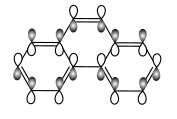
\includegraphics[scale=0.66]{./structures/exercise_1/phenanthrene/12.png}
			\captionof*{figure}{$\varepsilon = \alpha - 0.769\beta$}
			\end{minipage} & 
			\begin{minipage}[t]{0.21\linewidth}
			\setlength{\abovecaptionskip}{0.5em}
			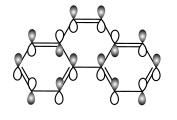
\includegraphics[scale=0.66]{./structures/exercise_1/phenanthrene/13.png}
			\captionof*{figure}{$\varepsilon = \alpha - 1.142\beta$}
			\end{minipage} &
			\begin{minipage}[t]{0.21\linewidth}
			\centering
			\setlength{\abovecaptionskip}{0.5em}
			\includegraphics[scale=0.66]{./structures/exercise_1/phenanthrene/5.png}
			\captionof*{figure}{$\varepsilon = \alpha - 1.306\beta$}
			\end{minipage} &
			\begin{minipage}[t]{0.21\linewidth}
			\setlength{\abovecaptionskip}{0.5em}
			\includegraphics[scale=0.66]{./structures/exercise_1/phenanthrene/6.png}
			\captionof*{figure}{$\varepsilon = \alpha - 1.516\beta$}
			\end{minipage} \\
			\begin{minipage}[t]{0.21\linewidth}
			\centering
			\setlength{\abovecaptionskip}{0.5em}
			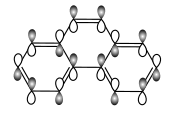
\includegraphics[scale=0.66]{./structures/exercise_1/phenanthrene/14.png}
			\captionof*{figure}{$\varepsilon = \alpha - 1.951\beta$}
			\end{minipage} & 
			\begin{minipage}[t]{0.21\linewidth}
			\setlength{\abovecaptionskip}{0.5em}
			\includegraphics[scale=0.66]{./structures/exercise_1/phenanthrene/7.png}
			\captionof*{figure}{$\varepsilon = \alpha - 2.435\beta$}
			\end{minipage} &
			\begin{minipage}[t]{0.21\linewidth}
			\end{minipage} &
			\begin{minipage}[t]{0.21\linewidth}
			\end{minipage} \\
		\end{tabular}				
		\captionof{figure}{Phase diagrams of these H{\"u}ckel MOs of phenanthrene. Black bubbles mean plus phase while white ones mean minus phase. The color is used just for determining relative phase.}\label{fig:phase_diagram_6}
		\end{center}
		
		In the end, we conclude that for phenanthrene, its ground state $\pi$-electron configuration is $(1b_1)^2 (1a_2)^2 (2b_1)^2 (3b_1)^2 (2a_2)^2 (3a_2)^2 (4b_1)^2$ and its delocalization energy is $2 \times 2.435 \beta + 2 \times 1.951 \beta + 2 \times 1.516 \beta + 2 \times 1.306 \beta + 2 \times 1.142 \beta + 2 \times 0.769 \beta + 2 \times 0.605 \beta - 14 \times 1.000 \beta = 5.448 \beta$, much larger than the sum of that of {\it trans}-1,3-butadiene ($0.472\beta$) and two benzenes ($2.000\beta \times 2$). 
		
		\begin{center}
		\includegraphics[scale=1.0]{./structures/exercise_1/phenanthrene/998.png}
		\end{center}
		
		\end{enumerate}	
		
	\end{solution}

\end{document}